
\chapter{Characterization of the Multilayer Structure for Different Systems} \label{ch_spec}
The multilayer mirror samples we shall investigate here were fabricated using the magnetron sputtering technique briefly discussed in the chapter~\ref{ch_exp} with nominal layer thicknesses and chemical species, depending on the desired reflection angle and spectral range. Among other parameters of the production process, the achieved individual layer thickness and morphology of the interfaces has a direct impact on the performance of these mirrors with respect to their peak reflectance and bandwidth. Although the sputtering process is a well established technique for mirror fabrication, the actual layer thicknesses in the sample may differ from the nominal values.

Based on the matrix algorithm introduced in chapter~\ref{ch_theo}, the electromagnetic fields   inside and outside an arbitrary layer system can be calculated. Most importantly, this allows to calculate the expected specular reflectance curves across angular or spectral ranges for a given layer model. The comparison of these calculated curves to measured data thus allows to obtain information about the actual layer properties in a given sample with a destruction free approach. However, the detected reflectance values in a specular reflection experiment do not contain the information on the phase of the electromagnetic wave, which is lost. It is thus not possible to directly reconstruct the layout of the sample with the measured reflection curve. This is known as the inverse problem of scatterometry. Reconstructing the layer properties is therefore an attempt of solving this inverse problem by accumulating prior knowledge about the sample, such as the nominal design goals during the fabrication process, into a model of that system. Starting from this model, the theoretically calculated curve is compared to the measured reflectance and optimized iteratively.

In order to add complementary information for refining the solution of the inverse problem, additional methods with sensitivities for different properties of the sample can be applied. In this chapter, depending on the sample system, we analyze several experimental methods. Apart from the aforementioned reflectance in the \gls{euv} spectral range, we apply resonant \gls{euv} reflectance across absorption edges, \gls{xrr} with high photon energy and finally \gls{xrf}. The latter does rely on the measurement of fluorescence radiation and thus requires the calculation of the field intensities inside the layer stack at the position of a specific chemical species for its analysis as described in section~\ref{ch_theo:sec_xrf} of chapter~\ref{ch_theo}.

% This chapter consists of three parts attributed to the study of three sample system categories. Firstly, the analysis of the specular \gls{euv} reflectance is applied and discussed in detail in section~\ref{ch_spec:sec_reconstruction_PTB17} to a high-reflectance multilayer mirror composed out of Mo/B$_4$C/Si/C optimized for reflection in the spectral range between $\lambda=\nm{12.4}$ and $\lambda=\nm{14.0}$ at angles of incidence below $\alpha_i \leq \SI{15}{\degree}$ based on the data at those wavelengths and angles.
% 
% Secondly, we apply the findings of the

% \begin{itemize}
%  \item more about what people already do
%  \item what are the problems (no unique solution)
%  \item solution approach: PSO
%  \item validation with MCMC and confidence intervals
%  \item combination of several methods to improve
%  \item for Cr/Sc: standard model does not work anymore, better model necessary
%  \item for Cr/Sc: how can better model be solved uniquely?
% \end{itemize}


\section{Reconstruction Based on Specular EUV reflectance} \label{ch_spec:sec_PTB17}
\label{ch_spec:sec_reconstruction_PTB17}
In this section we demonstrate the reconstruction of a multilayer system designed as near-normal incidence mirror for the wavelength range between \nm{12.4} and \nm{14.0} based solely on experimental data of \gls{euv} reflectivity. The mirror was designed to achieve a peak in the reflectance at a wavelength of $\lambda=\nm{13.5}$ for an angle of incidence of $\alpha_i = \SI{6}{\degree}$. That combination is of relevance for optical setups in the next generation lithography for the semiconductor industry, for which this sample served as a prototype. The multilayer coating was deposited with magnetron sputtering on a polished silicon substrate. The sample contains a periodic layer stack of molybdenum (Mo) and silicon (Si). Due to the problem of intermixing and resulting loss of interface definition, additional barrier layers of boroncarbite (B$_4$C) and carbon (C) were included at the Mo to Si and Si to Mo interfaces, respectively. We shall therefore refer to this sample with the layer sequence within one period from bottom to top as Mo/B$_4$C/Si/C. The periodicity of that system is $N=65$, while the $65th$ (capping) layer period does not posses a carbon layer but terminates at the vacuum interface with the silicon layer. A detailed schematic figure of the layer layout can be found in the description of the corresponding theoretical model in Fig.~\ref{ch_spec:fig_Mo_B4C_Si_C_model}.

The sample was measured with respect to its reflectivity across the spectral range mentioned above at an angle of incidence of $\alpha_i=\SI{15}{\degree}$ from the surface normal. The measurement was conducted at the \gls{euvr} beamline at the \gls{mls}. The reflectivity was evaluated by first measuring the intensity of the direct beam in the reflectometer with the photo diode detector. Then, the reflected radiation at an detector angle of $\SI{30}{\degree}$ was measured in reference to the direct beam signal. To ensure the stability of the result, the direct beam was measured again afterwards and compared to the data of the first measurement. The normalized results are shown in Fig.~\ref{ch_spec:fig_ptb17_reflectance_AOI_15}. The measurement uncertainty in with this experimental method is within $\SI{1}{\percent}$ of the peak reflectance value. Consequently, the error margin is within the line thickness of the data presentation in Fig.~\ref{ch_spec:fig_ptb17_reflectance_AOI_15}.
\begin{figure}[htbp]
\centering
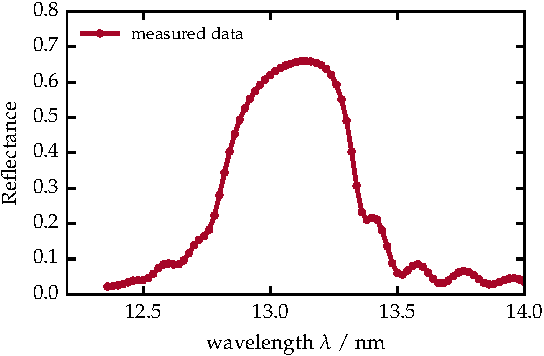
\includegraphics{img/PTB17_reflectance_AOI_15}
\caption{Spectrally resolved reflectance data of the Mo/B$_4$C/Si/C multilayer sample. The irradiation was conduced under a fixed angle of incidence $\alpha_i = 15.0^\circ$. The measurement uncertainty is within the line thickness of the plot.}
\label{ch_spec:fig_ptb17_reflectance_AOI_15}
\end{figure}

The reflectiviy curve shows a broad peak attaining its maximum value at a wavelength of approximately \nm{13.1}, which is lower than the design peak reflectance of \nm{13.5}. That is due to the different angle of incidence used in the experiment. Apart from the main peak, side fringes are visible. They originate due to a superposition of waves being reflected at the top surface and the substrate interface. They are thus directly related to the total thickness of the multilayer coating and well known as \emph{Kiessig fringes} \cite{kiessig_interferenz_1931}. Based on the data obtained through this spectrally resolved reflectivity experiment, we shall attempt to reconstruct the unknown layer layout in the following sections. The nominal fabrication parameters serve as starting values for the analysis to construct a reasonable model for the reconstruction.

The reconstruction of a given model based on the evaluation of \gls{euv} (or \gls{xrr}) reflectivity data is a well established method for the characterization of multilayer systems  \cite{lim_fabrication_2001, bajt_investigation_2001, braun_mo/si_2002}. In most cases a model is constructed and optimized applying gradient methods such as the Levenberg-Marquardt method \cite{levenberg_method_1944, marquardt_algorithm_1963}. Those optimization algorithms typically operate with a set of start parameters within the parameter space and iteratively improve the overlap of the prediction from the theoretical calculation and the experimental data. This is done by calculating the gradient of a minimization functional, usually termed $\chi^2$, in all directions in the parameter space and changing the parameters accordingly in direction of smaller $\chi^2$ values. This approach has the major disadvantage that the end result is strongly dependent on the choice of starting values and may not represent a global minimum of $\chi^2$ but only a local optimum. While estimations of the quality of the fit results within the (local) optimum are possible, no estimation can be given globally for the given model. For those reasons, this characterization strategy has only limited applicability and alternative approaches are required.

In contrast to those gradient methods, heuristic optimization algorithms exist. Instead of operating with predefined starting values, from which a gradient approach minimizes the $\chi^2$ functional, they operate distributed on the whole parameter space with often randomly initialized parameters within given boundaries, instead. In the following we shall apply those heuristic optimization routines to obtain the reconstruction of the Mo/B$_4$C/Si/C sample and elaborate their application to the characterization of multilayer systems in detail.

\subsection{Multilayer Model and Particle Swarm Optimization} \label{ch_spec:sec_multilayer_model_and_pso}
For the purpose of reconstructing the layer layout of the Mo/B$_4$C/Si/C sample, a parameterized model is needed entering the theoretical calculations to obtain the reflectivity curve according to the matrix algorithm. The model is largely based on prior knowledge available from the fabrication process. For the multilayer sample investigated here, the nominal layer design is known and a schematic representation is shown in Fig.~\ref{ch_spec:fig_Mo_B4C_Si_C_model}.
\begin{figure}[htbp]
    \def\svgwidth{0.7\textwidth}
    \fontfamily{fds}\selectfont\footnotesize
    \import{svg/}{mo_si_ptb17_model.pdf_tex}
    \caption{Model of the multilayer stack including the substrate and the capping layers. The periodic part is enclosed between the dashed lines with four layers in each period repeated $N=64$ times. The capping period does not include an interdiffusion layer but does reflect the natural oxidation through the addition of a SiO$_2$ layer.}
    \label{ch_spec:fig_Mo_B4C_Si_C_model}
\end{figure}
As introduced above, the multilayer coating consists of a periodic arrangement of four layers replicated 64 times. With the top period being different from the others through the missing carbon interdiffusion layer on the top surface. Since the sample was exposed to ambient conditions, a passivation of the top silicon surface through oxidation has to be taken into account through a silicondioxide layer. The parameterization of that model is given by the thicknesses of each layer within one period as well as for the capping silicondioxide layer. Each of the deposited layers may vary in density with respect to the bulk density of that material \cite{braun_mo/si_2002}, which also needs to be reflected in the model. Finally, the N{\'e}vot-Croce factor $\sigma$ accounting for roughness and interdiffusion at the interfaces as introduced in chapter \ref{ch_theo} is also included. The required optical constants, i.e.~the indices of refraction, of the respective materials in the relevant spectral range are taken from tabulated values by \textcite{henke_x-ray_1993} and used for the theoretical calculations based on the matrix algorithm. A full list of the model parameters for the multilayer sample can be found in table~\ref{ch_spec:tbl_mo_b4c_si_c_multilayer_parameters} together with physically plausible limits for each of the parameters. Due to the fact that the \gls{euv} reflectivity curve shown in Fig.~\ref{ch_spec:fig_ptb17_reflectance_AOI_15} shows the first order Bragg peak of the layer system, none of the layers can be thicker than \nm{7}, i.e.~in the order of half of the wavelength. The barrier layers were designed to attain thicknesses below \nm{1}. The densities of the various materials within this model was constrained to values between $\SI{50}{\percent}$ and $\SI{100}{\percent}$ with respect to their bulk density. This is introduced to take into account reduced layer densities due to possible intermixing during deposition. Through this, the bulk density may not be attained. A layer with a density above the bulk density, on the other hand, is unlikely. Due to the high peak reflectance close to the theoretical limit of the multilayer sample in the \gls{euv} measurement, the maximum value of the N{\'e}vot-Croce factor was limited to be below $\sigma \leq \nm{2}$. With its upper limit, the measured peak reflectance can not be attained within this model thus not limiting the generality.
\begin{table*}
\centering
\caption{Multilayer parametrization and parameter limits}
\label{ch_spec:tbl_mo_b4c_si_c_multilayer_parameters}
\begin{tabular}{@{}llll@{}}
\toprule
Parameter & Definition & Lower bound & Upper bound\\ \midrule
$d_\text{Mo}$ / nm & Mo layer thickness & $0.0$& $7.0$\\ 
$d_\text{Si}$ / nm & Si layer thickness& $0.0$& $7.0$\\ 
$d_\text{C}$ / nm &C buffer layer thickness& $0.0$ & $5.0$\\ 
$d_\text{B$_4$C}$ / nm &B$_4$C buffer layer thickness&$0.0$ & $5.0$\\ 
$\sigma$ / nm & N\'{e}vot-Croce parameter& $0.0$& $2.0$\\ 
&(identical for all interfaces)&&\\
$\rho_\text{Mo}$ &Mo density w.r.t.~bulk density & $0.5$& $1.0$\\ 
$\rho_\text{Si}$ &Si density w.r.t.~bulk density& $0.5$& $1.0$\\ 
$\rho_\text{C}$ &C density w.r.t.~bulk density& $0.5$& $1.0$\\ 
$\rho_\text{B$_4$C}$ &B$_4$C density w.r.t.~bulk density& $0.5$& $1.0$\\
\midrule
\multicolumn{4}{c}{Capping layer}\\
\midrule
$d_\text{SiO$_2$(cap)}$ / nm & SiO$_2$ capping layer thickness & $0.0$&$5.0$ \\ 
$\rho_\text{SiO$_2$(cap)}$& $=\rho_\text{Si}$ (identical to Si density)& & \\
 \bottomrule
\end{tabular}
\end{table*}

\paragraph{The minimization functional and particle swarm optimization}
As introduced above, the reconstruction of the model for the multilayer is an optimization problem. Based on the measured reflectivity data an optimization functional defines the goodness of the model with respect to the measured data. The quality is asserted based on the method of least squares \cite{legendre_nouvelles_1805, gauss_theoria_1809, birge_calculation_1932} and the functional is defined as the reduced $\tilde{\chi}^2$
\begin{align}
\tilde{\chi}^2 = \frac{1}{M-P} \bigg[\sum\limits_{m} \frac{(I_m^\text{model} 
- I_m^\text{meas})^2}{\tilde{\sigma}_m^2} \bigg] \text{,} 
\label{ch_spec:eqn_reduced_chi_squared}
\end{align}
where $M$ is the number of measurement points, $P$ is the number of parameters used in the model, $I_m^\text{model}$ is the calculated intensity for the corresponding measurement point with index $m$ having the measured intensity $I_m^\text{meas}$. The calculated intensity fur the \gls{euv} reflectivity curve above $I_m^\text{model}$ follows directly from the matrix algorithm and the quantity $R$ in Eq.~\eqref{ch_theo:eqn_refl_trans_ML} in chapter~\ref{ch_theo}. Each point is calculated based on the angle of incidence and wavelength associated with measurement point $m$. The experimental uncertainty for each measurement point is described by $\tilde{\sigma}_m$.

For the minimization of the functional in Eq.~\eqref{ch_spec:eqn_reduced_chi_squared} we apply a global optimization algorithm known as \gls{pso} \cite{kennedy_particle_2011}. In contrast to the aforementioned gradient based methods, the particle swarm optimizer operates on the whole parameter space as defined by the upper and lower parameter limits, which are given in table~\ref{ch_spec:tbl_mo_b4c_si_c_multilayer_parameters} for the particular example here, without specific starting parameters influencing the convergence result. We implemented the \gls{pso} algorithm based on the draft by \textcite{carlisle_off--shelf_2001}. The basic mechanism of the algorithm is the definition of a swarm of individual particles, which are initialized randomly distributed across the allowed parameter space. Initially, each of those particles calculates the minimization functional at its random position retaining that result including a random start velocity. In an iterative process, the global best solution (``social component'') found as well as the individual best solution (``cognitive component'') of each particle are used to calculate an updated and weighted velocity vector within the parameter space for each particle. Within that iteration each of the particle thus moves to a new position, where the minimization functional is again evaluated and compared the the individual and global best solutions. If a better value is found, the respective retained results are updated with the new value and the next iteration is performed. While following that process the particles eventually converge to the global best solution, which may or may not be the global best optimum of the whole optimization problem. Due to the combination of social and cognitive component, fast convergence into a local optimum can be avoided. The state of full convergence is reached, when either all particles occupy the same place in the parameter space or if stagnation is reached. Due to the heuristic nature of the algorithm, it may happen that the global best optimum found is not necessarily the global minimum of the optimization problem. The result may be verified, however, by repeated application of the algorithm or simply by reaching a satisfactory solution through comparison of the measured and calculated curves and thus small $\tilde{\chi}^2$ values.

\paragraph{Model reconstruction based on the \gls{euv} reflectivity data}
We have applied this optimization procedure to the Mo/B$_4$C/Si/C sample and the measured \gls{euv} reflectivity curve. The fit result is shown together with the measured data in Fig.~\ref{ch_spec:fig_ptb17_reflectance_AOI_15_fitted}.
\begin{figure}[htbp]
\centering
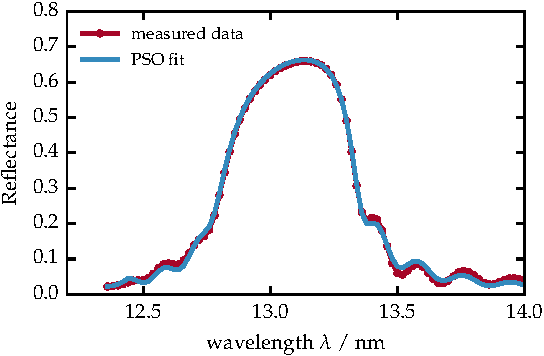
\includegraphics{img/PTB17_reflectance_AOI_15_fitted}
\caption{Theoretical reflectance curve based on the optimal model parameters obtained from the particle swarm optimization.}
\label{ch_spec:fig_ptb17_reflectance_AOI_15_fitted}
\end{figure}
The parameter results are listed in table~\ref{ch_spec:tbl_mo_b4c_si_c_multilayer_parameters_results}. The solution does indeed provide a very good agreement with the measured data. However, by repeated evaluation of the \gls{pso} procedure, significantly different results for the optimal parameter set with comparable agreement and very similar $\chi^2$ values were found. Clearly, this is no desirable situation, since no definite answer of the actual thicknesses found in the sample can be made. To complete the characterization additional methods of model verification are thus required. We shall therefore discuss an additional approach to the optimization problem in the following section on how the model validity and the information content of the measured data can be asserted based on the example of the \gls{pso} results obtained here.
\begin{table}[htbp]
\centering
\caption{Results for the optimized parameters based on the \gls{pso} of the \gls{euv} reflectivity for the Mo/B$_4$C/Si/C sample.}
\label{ch_spec:tbl_mo_b4c_si_c_multilayer_parameters_results}
\begin{tabular}{@{}lll@{}}
\toprule
Parameter & Definition& PSO result\\ \midrule
$d_\text{SiO$_2$(cap)}$ / nm &SiO$_2$ capping layer thickness& $3.194$ \\
$d_\text{Mo}$ / nm &Mo layer thickness&  $2.460$ \\
$d_\text{Si}$ / nm &Si layer thickness& $2.421$\\ 
$d_\text{C}$ / nm &C buffer layer thickness& $0.811$\\ 
$d_\text{B$_4$C}$ / nm &B$_4$C buffer layer thickness& $1.308$\\ 
$\sigma$ / nm &N\'{e}vot-Croce parameter& $0.322$\\
$\rho_\text{Mo}$ &Mo density w.r.t.~bulk density& $0.989$\\ 
$\rho_\text{Si}$ &Si density w.r.t.~bulk density& $0.883$\\ 
$\rho_\text{C}$ &C density w.r.t.~bulk density& $0.833$\\ 
$\rho_\text{B$_4$C}$ &B$_4$C density w.r.t.~bulk density& $0.909$ \\
 \bottomrule
\end{tabular}
\end{table}

\subsection{Model Uniqueness and Maximum Likelihood Estimation} \label{ch_spec:sec_maximum_likelihood}
With the ambiguous reconstruction result of the previous section, the demand for a verification of the model with respect to the measured data becomes apparent. To clarify the problem of uniqueness of the solution, it is instructive to investigate the influence of the individual model parameters on the theoretical reflectivity curve. In Fig.~\ref{ch_spec:fig_mo_si_parameter_influence} we varied a subset of the parameters starting from the \gls{pso} solution from Sec.~\ref{ch_spec:sec_multilayer_model_and_pso}. In each of the subfigures, one parameter or a quotient of parameters is varied while all others are kept fixed.
\begin{figure*}[htbp]
\centering
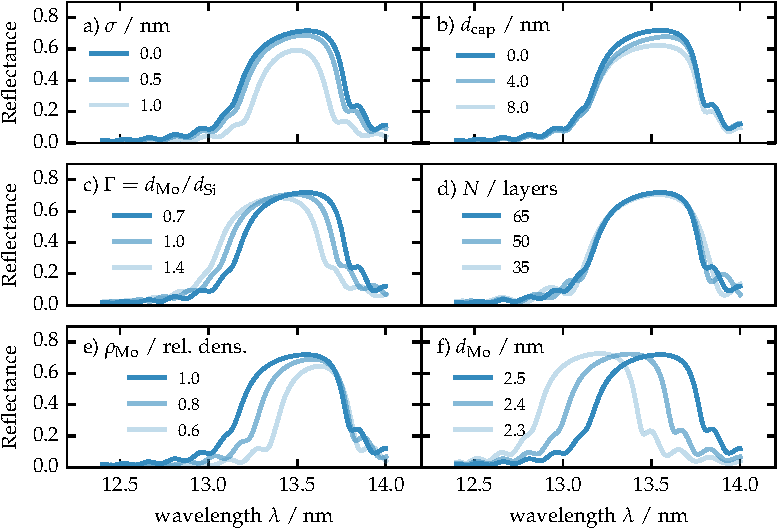
\includegraphics{img/parameter_influence}
\caption{Influence of the change of parameter model on the simulated \gls{euv} reflectivity curve. In each of the figures, all parameters were kept constant at the values listed in table~\ref{ch_spec:tbl_mo_b4c_si_c_multilayer_parameters_results} varying only the respective shown parameter.}
\label{ch_spec:fig_mo_si_parameter_influence}
\end{figure*}
By comparison of Fig.~\ref{ch_spec:fig_mo_si_parameter_influence}a, \ref{ch_spec:fig_mo_si_parameter_influence}b, \ref{ch_spec:fig_mo_si_parameter_influence}c and \ref{ch_spec:fig_mo_si_parameter_influence}e it becomes clear that a reduction of the peak reflectivity can originate in either a large roughness and interdiffusion parameter $\sigma$ or similarly from the thickness of the capping layer, the silicon to molybdenum layer thickness ratio of the molybdenum density. A reconstruction based on a single \gls{euv} reflectivity therefore intrinsically produces a highly ambiguous result with strong parameter correlations. The available data, a single \gls{euv} reflectivity curve in this case, does not allow for a unique set of parameters of the model minimizing the $\chi^2$ functional. In reality multiple solutions with very similar values for $\tilde{\chi}^2$ exist. Clearly, this raises the question of how accurately a reconstruction may be achieved here and requires to determine the value of $\tilde{\chi}^2$ in vicinity of the \gls{pso} solution or possibly the whole parameter space.

\paragraph{Maximum likelihood}
We approach this problem of evaluating $\tilde{\chi}^2$ across the parameter space by numerically sampling the functional based on a \gls{mcmc} method \cite{goodman_ensemble_2010}. An application of this technique to the design process of multilayer mirrors has been demonstrated by \textcite{hobson_markov-chain_2004}. In our case, the match of model and experimental result is evaluated based on a non-centered $\chi^2$ distribution assuming independent measurements. We further assume that any measured point is distributed around the actual reflectivity curve following a Gaussian distribution, i.e.~we assume Gaussian uncertainties for the experiment. The corresponding probability density function for a measurement result matching with the actual reflectivity curve, which is assumed to be obtainable exactly through the theoretical calculation, is then of Gaussian form \cite{abramowitz_handbook_1964}. Thus, the likelihood that the measured values match with the theoretical curve under the assumption that the model is correct is proportional to
\begin{align}
 L(E | M(\vec{x})) \propto \exp \big(- \tilde{\chi}^2(\vec{x}) / 2 \big) \text{,} \label{ch_spec:eqn_likelihood_experiment_vs_model}
\end{align}
where $E$ denotes the experiment, i.e.~the measured data and $M(\vec{x})$ represents the model given through parameter set $\vec{x}$, e.g.~the parameters of the model in table~\ref{ch_spec:tbl_mo_b4c_si_c_multilayer_parameters}. In our case however, we seek to evaluate the likelihood $L(M(\vec{x}) | E)$ that the model $M(\vec{x})$ with a given set of parameters $\vec{x}$ is valid assuming the experiment $E$ yields the correct curve (the so called ``posterior distribution''). Those two quantities are linked through the Bayesian theorem \cite{bayes_essay_1763, milton_introduction_2002} stating
\begin{align}
 L(M(\vec{x}) | E) \propto L(E | M(\vec{x})) L(M(\vec{x})) \text{,} \label{ch_spec:eqn_bayesian_theorem}
\end{align}
where $L(M(\vec{x}))$ denotes the likelihood for the model to be valid for a specific set of parameters $\vec{x}$ (the so called ``prior distribution''). The prior distribution does contain any prior knowledge about the model and allowed parameters. For the example of the model parameters in table~\ref{ch_spec:tbl_mo_b4c_si_c_multilayer_parameters}, the prior distribution is $L(M(\vec{x})) \rightarrow -\infty$ for any parameter set outside the listed boundaries and $L(M(\vec{x})) = 1$ everywhere else. In addition, we limit the maximum total period thickness, i.e.~the sum of all layers in one period to only allow the appearance of the first Bragg peak within the measured spectral range through the same condition. Combining Eq.~\eqref{ch_spec:eqn_likelihood_experiment_vs_model} and Eq.~\eqref{ch_spec:eqn_bayesian_theorem} then yields the likelihood functional
\begin{align}
 L(\vec{x}) = L(M(\vec{x}) | E) \propto \exp \big(- \tilde{\chi}^2(\vec{x}) / 2 \big) L(M(\vec{x})) \text{.} \label{ch_spec:eqn_likelihood}
\end{align}

Solving the optimization problem posed in the previous section within this context is then, equivalently to the minimization of $\tilde{\chi}^2$, the maximization of the likelihood $L(\vec{x})$. The \gls{mcmc} method poses a statistical approach on evaluating (mapping) the likelihood across the parameter space within the previously defined limits as in the \gls{pso} approach. It thus yields an alternative method on solving the optimization problem by extracting the maximum likelihood from the final result. However, in addition to the maximum value, the likelihood distribution in parameter space is obtained allowing to extract confidence intervals for each of the parameters \cite{cox_theoretical_1979}. Thereby, the aforementioned ambiguity of solutions can be quantified within the defined model and the available experimental data. The confidence intervals are defined as the one- or two-sigma standard deviations of the respective distributions for each parameter.

\paragraph{Confidence intervals for the Mo/B$_4$C/Si/C sample}
We have applied an existing implementation of the \gls{mcmc} algorithm by \textcite{foreman-mackey_emcee:_2013} to the \gls{euv} measurement of the Mo/B$_4$C/Si/C sample in Fig.~\ref{ch_spec:fig_ptb17_reflectance_AOI_15} with the model in Fig.~\ref{ch_spec:fig_Mo_B4C_Si_C_model}. The likelihood, as defined in Eq.~\eqref{ch_spec:eqn_likelihood} with the $\tilde{\chi}^2$ functional from Eq.~\eqref{ch_spec:eqn_reduced_chi_squared}, is sampled in a high-dimensional space depending on the number of parameters in the model. We therefore need to project the distribution for each parameter by marginalizing over all other parameters. Alternatively, two-parameter correlations can be visualized by projecting on a two-dimensional area, again marginalizing across all other parameters. The projection for the Si and Mo layer thicknesses are shown in Fig.~\ref{ch_spec:fig_ptb17_MCMC_d_Mo_vs_d_Si}b and \ref{ch_spec:fig_ptb17_MCMC_d_Mo_vs_d_Si}c. In both cases, a well defined distribution is obtained. In the two-dimensional projection in Fig.~\ref{ch_spec:fig_ptb17_MCMC_d_Mo_vs_d_Si}a, no correlations are apparent and a two-dimensional Gaussian-like shape results.
\begin{figure*}[htbp]
\centering
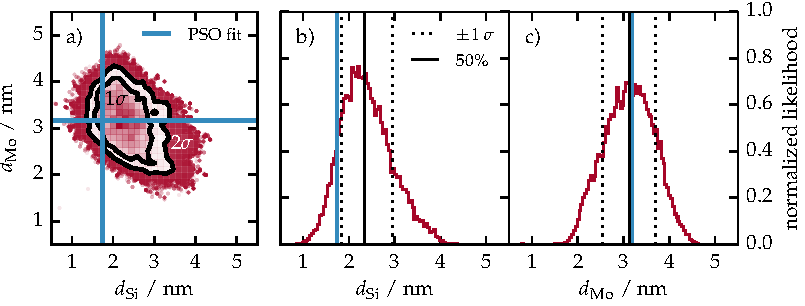
\includegraphics{img/PTB17_MCMC_d_Mo_vs_d_Si}
\caption{Results of the maximum likelihood estimation obtained via the \gls{mcmc} procedure. a) Two dimensional projection of the likelihood distribution for the parameter pair $d_\text{Si}$ and $d_\text{Mo}$. The projection was obtained by marginalizing over all other parameters of the model. The black contours indicate the areas for one and two standard deviations (one and two sigma contours). The blue lines in all three sub-figures indicate the best parameter set found with the \gls{pso} method. b) One dimensional projection of the likelihood distribution for the silicon layer thickness $d_\text{Si}$. The solid black line marks the center position ($50\%$ percentile) of the distribution. The dotted lines are the limits of one standard deviation. c) The one dimensional distribution similarly to b) for the molybdenum layer thickness.}
\label{ch_spec:fig_ptb17_MCMC_d_Mo_vs_d_Si}
\end{figure*}
\begin{figure*}[htbp]
\centering
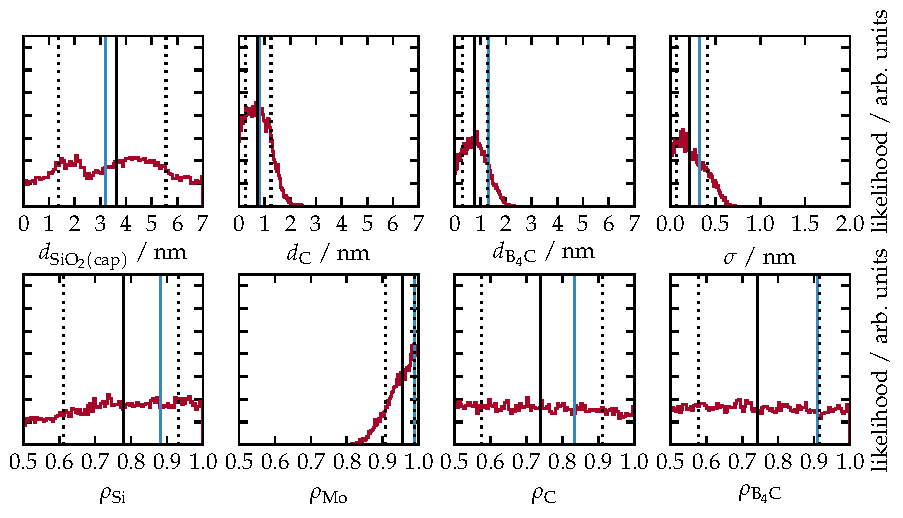
\includegraphics{img/PTB17_MCMC_other_params}
\caption{In analogy to Fig.~\ref{ch_spec:fig_ptb17_MCMC_d_Mo_vs_d_Si}b and \ref{ch_spec:fig_ptb17_MCMC_d_Mo_vs_d_Si}c the one dimensional projections of the likelihood distribution estimation for the Mo/B$_4$C/Si/C sample are shown for the remaining parameters of the model with the \gls{pso} result, the center value and one standard deviation.}
\label{ch_spec:fig_ptb17_MCMC_other_params}
\end{figure*}
In all cases, the one-sigma standard deviations for Gaussian distributions are shown together with the weighted center, i.e.~the $50$th percentile. The \gls{pso} result is also indicated, which is compatible with the one sigma standard deviation, but does not match the center of the likelihood result. The reason for that lies in higher order correlations of the parameters. In Fig.~\ref{ch_spec:fig_ptb17_MCMC_other_params}, all one-dimensional projections of the likelihood distribution are shown for all remaining parameters. Clearly, while a reasonably small confidence interval (again, one standard deviation for all distributions) can be found for the thickness of the carbon and boroncarbite layers, the off-center value for the silicon thickness of the PSO result in Fig.~\ref{ch_spec:fig_ptb17_MCMC_d_Mo_vs_d_Si}c is compensated by a larger than center value for the boroncarbite layer in Fig.~\ref{ch_spec:fig_ptb17_MCMC_other_params}. Thus, the thicknesses are correlated and are no independent model parameters. Nevertheless, confidence intervals can be obtained within the given model and the given prior (the boundaries listed in table~\ref{ch_spec:tbl_mo_b4c_si_c_multilayer_parameters}) and are listed accordingly in table~\ref{ch_spec:tbl_mo_b4c_si_c_multilayer_mcmc_results} for one and two standard deviations. Within the allowed boundaries, some parameters remain entirely undefined with similar likelihood for any parameter value, such as the SiO$_2$ capping layer thickness, the silicon, carbon and boroncarbite relative densities. Their corresponding total confidence intervals thus cover almost exactly $68.2\%$ (one standard deviation) and $95.4\%$ (two standard deviations) of the allowed respective parameter range. Hence, with respect to the model defined and the measured \gls{euv} reflectivity curve, no reliable value for those sample properties can be reconstructed.
\begin{table*}[htbp]
\centering
\caption{\gls{mcmc} results obtained by the analysis of the \gls{euv} reflectivity for the Mo/B$_4$C/Si/C sample. The center values ($50\%$ percentile) together with confidence intervals (c.i.) of one and two standard deviations are shown.}
\label{ch_spec:tbl_mo_b4c_si_c_multilayer_mcmc_results}
\begin{tabular}{@{}llll@{}}
\toprule
Parameter & PSO result & center value with $1 \sigma$ c.i.& center value with $2 \sigma$ c.i.\\ \midrule
$d_\text{SiO$_2$(cap)}$ / nm & $3.194$& $3.677({-2.252}/{+1.944})$ & $3.677({-3.407}/{+3.108})$ \\
$d_\text{Mo}$ / nm &  $2.460$& $3.137({-0.587}/{+0.560})$ & $3.137({-1.054}/{+1.016})$ \\
$d_\text{Si}$ / nm & $2.421$& $2.338({-0.497}/{+0.616})$ & $2.338({-0.916}/{+1.294})$ \\
$d_\text{C}$ / nm& $0.811$ & $0.744({-0.477}/{+0.510})$ & $0.744({-0.696}/{+0.971})$ \\
$d_\text{B$_4$C}$ / nm & $1.308$& $0.782({-0.471}/{+0.511})$ & $0.782({-0.722}/{+0.973})$ \\
$\sigma$ / nm & $0.322$& $0.214({-0.143}/{+0.201})$ & $0.214({-0.204}/{+0.347})$\\
$\rho_\text{Mo}$ & $0.989$& $0.953({-0.048}/{+0.034})$ & $0.953({-0.094}/{+0.045})$ \\
$\rho_\text{Si}$ & $0.883$& $0.782({-0.167}/{+0.147})$ & $0.782({-0.264}/{+0.208})$ \\
$\rho_\text{C}$ & $0.833$& $0.739({-0.164}/{+0.175})$ & $0.739({-0.228}/{+0.249})$ \\
$\rho_\text{B$_4$C}$ & $0.909$& $0.741({-0.162}/{+0.172})$ & $0.741({-0.230}/{+0.247})$ \\
 \bottomrule
\end{tabular}
\end{table*}

It should be noted, that although the aforementioned density values can not be determined based on the available data, they remain possibly highly correlated parameters. A valid optimization result can therefore only be obtained by either applying the \gls{pso} routine or by iterative application of the \gls{mcmc} procedure, fixing single parameters according to their maximum likelihood value in the model and obtaining the resulting likelihood distributions for the remaining parameters according to that restricted model.

The results listed in table~\ref{ch_spec:tbl_mo_b4c_si_c_multilayer_mcmc_results} serve as the model parameters for the analysis of diffuse scattering from the Mo/B$_4$C/Si/C sample in chapter~\ref{ch_diff}.

\section{Molybdenum Thickness Variation in Mo/Si/C Multilayers} \label{ch_spec:sec_mo_si_c}
In the following we shall apply and extend the reconstruction procedure discussed in the above section to the problem of multilayer sample systems deposited with varying molybdenum layer thicknesses from sample to sample. For the engineering of a near-normal incidence mirror, the ratio of molybdenum layer thickness to total period thickness has a clear impact on the reflectivity curve as seen in Fig.~\ref{ch_spec:fig_mo_si_parameter_influence}c. Studies have shown, that an optimal value for high reflectivity is achieved by depositing $40\%$ molybdenum layer thickness $d_\text{Mo}$ with respect to the total period thickness $D$ \cite{bajt_investigation_2001,braun_mo/si_2002}. During the deposition process, the layer of molybdenum grows in thickness and at a certain threshold, crystallites may begin to form \cite{verhoeven_ion_1992,bajt_investigation_2001} inside the layer. Those may affect the interface morphology of the layer system at the boundaries to the molybdenum layer and possibly at further interfaces through correlation effects. This potentially increases the roughness and thus the loss of specularly reflected radiation. For the deeper understanding of those effects, we shall reconstruct the layer structure and determine the molybdenum layer thickness in each sample in comparison to the nominal values for the magnetron sputtering deposition.

\subsection{Sample systems and experimental procedure}
As a specific prototype for high-reflectance multilayer mirrors for the \gls{euv} spectral range serve two sets of several samples of Mo/Si/C multilayer systems with C interdiffusion barriers with thicknesses of nominally below \nm{0.5} at the Mo on Si interfaces (a detailed figure of the model for those samples is given below in Fig.~\ref{ch_spec:fig_model_unpolished_and_polished_samples} of the following sections). As mentioned above, the samples under investigation here were fabricated with increasing relative Mo thickness from sample to sample while keeping the nominal period thickness $D\approx 7$ nm constant. In this study, we investigate two sets of samples. In the first set, the magnetron sputtered layers were deposited one after another for each sample. In the second set, during deposition, an additional polishing process was used once during sputtering each period to counteract the possible roughening due to the crystallization. The nominal values of the molybdenum layers in the two sample sets are listed in table~\ref{ch_spec:tbl_mo_si_thickness_nominal}.
\begin{table}[htbp]
\centering
\caption{List of nominal molybdenum layer thicknesses in the two sample sets. Both sets were fabricated with a equidistant increase in thickness from \nm{1.70} to \nm{3.05} with 9 unpolished and 10 polished samples.}
\label{ch_spec:tbl_mo_si_thickness_nominal}
\begin{tabular}{@{}ll@{}}
\toprule
nominal $d_\text{Mo}$ / nm & nominal $d_\text{Mo}$ / nm\\ 
(unpolished samples) & (polished samples) \\
\midrule
$1.70$& $1.70$\\ 
$1.85$& $1.85$\\ 
$2.00$ & $2.00$\\ 
$2.15$ & $2.15$\\ 
$2.30$& $2.30$\\ 
$2.45$& $2.45$\\ 
$2.60$& $2.60$\\ 
$2.75$ & $2.75$\\ 
$2.90$ & $2.90$\\ 
-& $3.05$\\ 
 \bottomrule
\end{tabular}
\end{table}

Spectrally resolved \gls{euv} reflectivity curves at an angle of incidence from the surface normal of $\alpha_i=\SI{15}{\degree}$ and in the wavelength range from \nm{12.4} to \nm{14.0} have been measured for all samples at the \gls{euvr} beamline at the \gls{mls}. The data obtained is shown in Fig.~\ref{ch_spec:fig_EUV_reflectivity_unpolished_and_polished} sorted by the nominal molybedum layer thickness.
\begin{figure}[htbp]
\centering
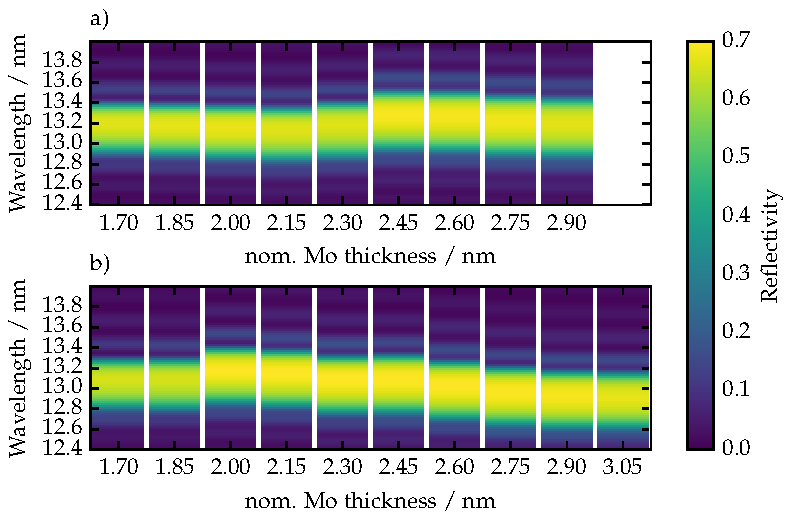
\includegraphics[width=0.7\textwidth]{img/MoSi_EUV_reflectivity}
\caption{a) Measured reflectivity curves for the unpolished samples across the wavelength at a fixed angle of incidence of $\alpha_i = 15^\circ$ from the surface normal. The nine samples differ by the nominal Mo layer thickness indicated at the bottom axis. b) Measured reflectivity curves of the ten polished samples measured under the same conditions as for the first sample set.}
\label{ch_spec:fig_EUV_reflectivity_unpolished_and_polished}
\end{figure}
The reflectivity curves in Fig.~\ref{ch_spec:fig_EUV_reflectivity_unpolished_and_polished}a and Fig.~\ref{ch_spec:fig_EUV_reflectivity_unpolished_and_polished}b have the characteristic curve shape of periodic \gls{euv} multilayer mirrors with a main broad maximum and side fringes, very similar to the mirror sample discussed in Sec.~\ref{ch_spec:sec_PTB17} above. In direct comparison of the measured reflectivity data, shifts of the peak center position are clearly visible. As illustrated in Fig.~\ref{ch_spec:fig_mo_si_parameter_influence} above, several properties of a multilayer stack, e.g.~molybdenum content and period thickness, contribute to such a difference. Clear differences in the peak reflectance value can also be observed in the two subfigures, with strong increases at $d_\text{Mo}^\text{nom} = \nm{2.45}$ for the unpolished set and at $d_\text{Mo}^\text{nom} = \nm{2.00}$ for the polished set. In all samples the only nominal difference, i.e.~the only parameter changed during the deposition process, is the relative molybdenum thickness. The increase in reflectance, peak broadening and the jump of the peaks center position are therefore indicators for an abrupt change in the multilayer properties.

For the purpose of obtaining additional information about the samples, in addition to the \gls{euv} reflectivity curves above, all samples were measured after deposition using a lab-based Cu-K$_\alpha$ X-ray diffractometer at the Fraunhofer IWS Dresden, Germany. The \gls{xrr} data is shown in Fig.~\ref{ch_spec:fig_MoSi_XRR} for the set of unpolished and polished samples in direct comparison.
\begin{figure*}[htbp]
\centering
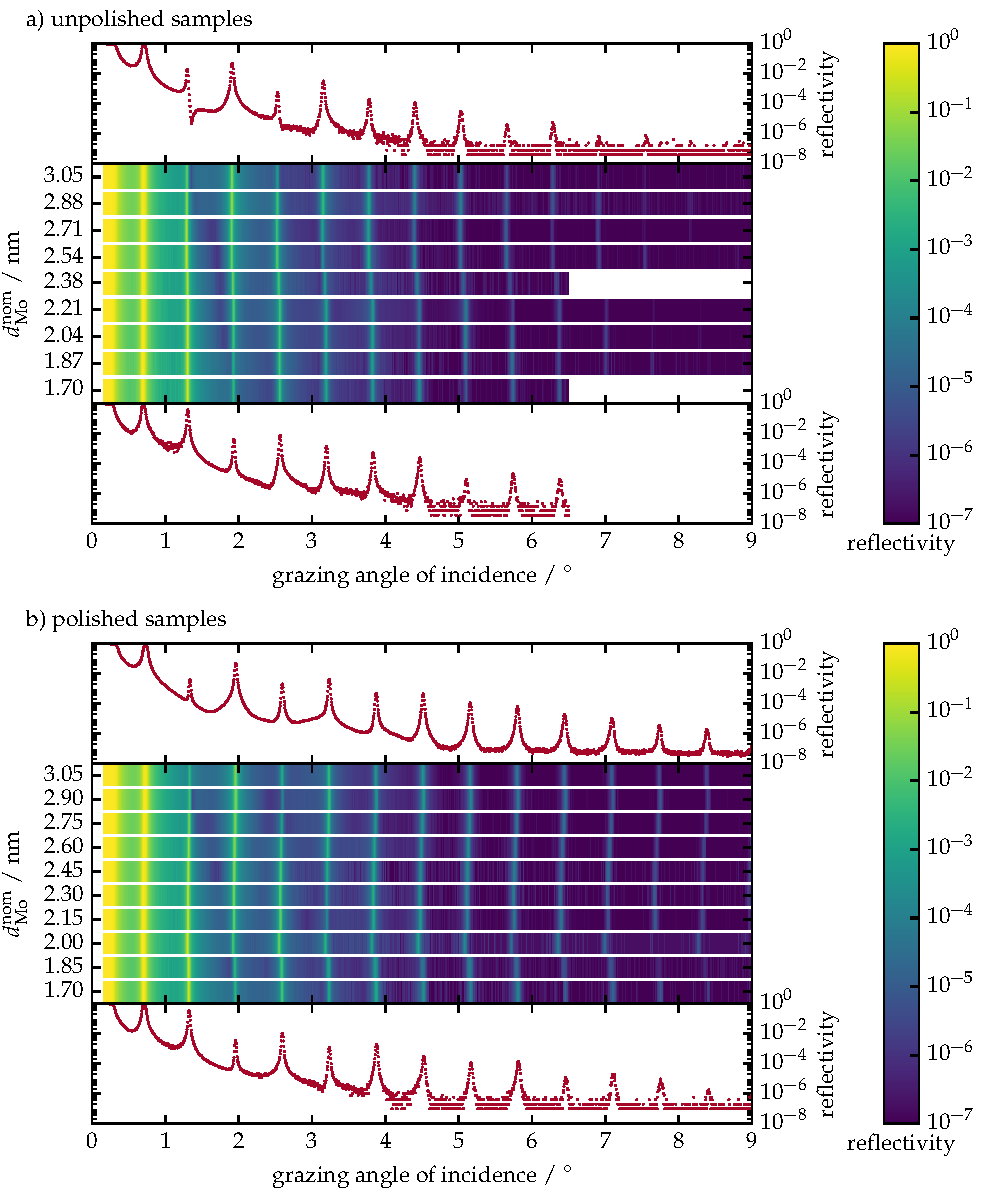
\includegraphics[width=\textwidth]{img/XRR_MoSi}
\caption{\gls{xrr} data for all unpolished and polished samples shown in dependence on the nominal molybdenum layer thickness $d_\text{Mo}^\text{nom}$ and the grazing angle of incidence $\alpha_i^\text{GI}$ at the Cu-K$_\alpha$ photon energy of $E_\text{ph} = \ev{8048}$. In each of the subfigures a) and b) the \gls{xrr} measurements for the sample with smallest and largest $d_\text{Mo}^\text{nom}$ are shown on the bottom and the top of the subfigure, respectively. In between, the \gls{xrr} curves are shown in as a color map plot.}
\label{ch_spec:fig_MoSi_XRR}
\end{figure*}
The position of the Bragg peaks and their respective intensity contain additional information on the layer stack thicknesses and its interface properties. In both cases, shifts of the peak positions and intensities similar to those observed in the \gls{euv} curves become apparent. Especially the higher orders towards larger grazing incidence angles show distinct differences. In addition, in direct comparison of the \gls{xrr} curves for the respective sample with $d_\text{Mo}^\text{nom} = \nm{3.05}$ from the unpolished and polished sets (on the top of Fig.~\ref{ch_spec:fig_MoSi_XRR}a and Fig.~\ref{ch_spec:fig_MoSi_XRR}b), a higher intensity for higher-order Bragg peaks above grazing angles of incidence of $\alpha_i^\text{GI} > \SI{7}{\degree}$ can be observed for the polished sample. This hints towards an improved interface definition and sharpness due to the polishing process and consequently a lower roughness or interdiffusion.

In the following section we shall analyze the \gls{euv} and \gls{xrr} data discussed here to reconstruct a model of the samples using the \gls{mcmc} approach introduced in Sec.~\ref{ch_spec:sec_reconstruction_PTB17} in order to verify the observations made here.

\subsection{Combined Analysis of X-ray and EUV reflectance} \label{ch_spec:sec_MoSi_euv_xrr_combined}
To obtain the actual layer thicknesses in the samples, we analyzed the data of the \gls{euv} reflectivity and \gls{xrr} experiments and reconstructed these parameters by combined analysis of the measured data. The reflectivity curves for the different measurements are calculated by introducing a model for the multilayer system and applying the matrix formalism described in detail in the theory part of this thesis, Sec.~\ref{ch_theo:sec_matrix_algorithm}.

The thicknesses of the Mo layers inside the stack were varied nominally from $1.7$ nm to $3.05$ nm from sample to sample, where the unpolished sample set lacks the last nominal thickness. The stacking of the different layers in the multilayer consists of the Mo and Si layers, as well as an additional C buffer layer at the Mo on Si interface to prevent interdiffusion. For the Si on Mo interfaces, no buffer layers were included since interdiffusion is usually less in this case \cite{petford-long_highresolution_1987}. However, for the theoretical description of the sample stack we consider an additional MoSi$_2$ layer in the model, which is well known to form during the deposition process \cite{bajt_investigation_2001}. The full model used in the reconstruction is illustrated in Fig.~\ref{ch_spec:fig_model_unpolished_and_polished_samples} with the thickness parameters for each layer.
\begin{figure}[htbp]
    \def\svgwidth{0.7\textwidth}
    \fontfamily{fds}\selectfont\footnotesize
    \import{svg/}{mo_si_iws_model.pdf_tex}
    \caption{Model of the multilayer stack including the substrate and the capping layers. The periodic part is enclosed between the dashed lines with four layers in each period repeated 49 times. The capping period does not include an interdiffusion layer but has a natural SiO$_2$ layer and a carbon-like layer accounting for contamination on the top surface.}
    \label{ch_spec:fig_model_unpolished_and_polished_samples}
\end{figure}
To account for any contamination on the top sample surface, an additional carbon-like layer as the upper most layer was considered. In addition to the thicknesses of each layer we also allowed for a variation of the layer density between $80\%$ and $100\%$ of the bulk density. The model parameters and their boundaries entering in the optimization procedure are listed in table~\ref{ch_spec:tbl_mo_si_c_multilayer_parameters}. Similar to the Mo/B$_4$C/Si/C in Sec.~\ref{ch_spec:sec_reconstruction_PTB17}, a N\'{e}vot-Croce damping factor was assumed to account for specular reflectivity loss due to interface imperfections. 
\begin{table*}
\centering
\caption{Parametrization of the Mo/Si/C multilayer samples with varying molybdenum layer thicknesses.}
\label{ch_spec:tbl_mo_si_c_multilayer_parameters}
\begin{tabular}{@{}llll@{}}
\toprule
Parameter & Definition & Lower bound & Upper bound\\ \midrule
$d_\text{Mo}$ / nm & Mo layer thickness & $0.0$& $4.5$\\ 
$d_\text{Si}$ / nm & Si layer thickness& $0.0$& $7.0$\\ 
$d_\text{C}$ / nm &C buffer layer thickness& $0.0$ & $0.6$\\ 
$d_\text{MoSi$_2$}$ / nm &MoSi$_2$ interdiffusion layer thickness&$0.0$ & $0.6$\\ 
$\sigma$ / nm & N\'{e}vot-Croce parameter& $0.0$& $0.5$\\ 
&(identical for all interfaces)&&\\
$\rho_\text{Mo}$ &Mo density w.r.t.~bulk density & $0.8$& $1.0$\\ 
$\rho_\text{Si}$ &Si density w.r.t.~bulk density& $0.8$& $1.0$\\ 
$\rho_\text{C}$ &C density w.r.t.~bulk density& $0.8$& $1.0$\\ 
$\rho_\text{MoSi$_2$}$ &MoSi$_2$ density w.r.t.~bulk density& $0.8$& $1.0$\\
\midrule
\multicolumn{4}{c}{Capping layer}\\
\midrule
$d_\text{C(cap)}$ / nm & C capping layer thickness & $0.0$&$3.0$ \\ 
$d_\text{SiO$_2$(cap)}$ / nm & SiO$_2$ capping layer thickness & $0.0$&$1.5$ \\ 
$\rho_\text{C(cap)}$ &C density w.r.t.~bulk density& $0.0$& $1.0$\\ 
$\rho_\text{SiO$_2$(cap)}$& $=\rho_\text{Si}$ (identical to Si density)& & \\
 \bottomrule
\end{tabular}
\end{table*}

\paragraph{Optimization functional and procedure}
The data analysis was conduced similarly to the procedure described in Sec.~\ref{ch_spec:sec_reconstruction_PTB17}. However, for the samples studied here, data from two seperate experiments was measured with the goal to improve the reconstruction of the model. Due to the increased amount of data through the additional \gls{xrr} measurements, a definition for a combined $\chi^2$ functional is required to allow an analysis based on both data sets. The two data sets, i.e.~the \gls{euv} and \gls{xrr} reflectivity curves have significantly different number of data points, which are not entirely independent of each other. In case of the \gls{xrr} curve increasing the number of data points, e.g.~by reducing the angular step size by half does not lead to better statistics due to systematic errors. Defining a $\chi^2$ functional as the total sum of all measured data point residuals, i.e.~both the \gls{euv} data and the \gls{xrr} data would therefore create an unwanted weighting due to the large amount of \gls{xrr} data points in comparison to far fewer \gls{euv} data points. To avoid this effect, we define the combined $\chi^2$ functional as the sum of the reduced $\tilde{\chi}^2$ functionals. The $\tilde{\chi}^2$ is equivalently defined to Eq.~\eqref{ch_spec:eqn_reduced_chi_squared} through,\begin{align}
\tilde{\chi}^2 = \frac{1}{M-P} \bigg[\sum\limits_{m} \frac{(I_m^\text{model} 
- I_m^\text{meas})^2}{\tilde{\sigma}_m^2} \bigg] \text{,}
\end{align}
for each of the datasets separately. The reduced $\tilde{\chi}^2$ can be interpreted as the average of the squared residuals of model prediction and experiment. Thereby, each experiment is reduced to a single comparable quantity. By the definition of
\begin{align}
\chi^2 = \tilde{\chi}^2_\text{EUV} +\tilde{\chi}^2_\text{XRR} \text{,}
\label{ch_spec:eqn_Mo_Si_C_total_chi_2}
\end{align}
we are therefore enabled to obtain confidence intervals for the parameters of the model, which represent a conservative (upper limit) estimation for the combined analysis of both experiments, similarly to the procedure for a single \gls{euv} curve as described in Sec.~\ref{ch_spec:sec_reconstruction_PTB17} above. The combined $\chi^2$ functional enters the likelihood through Eq.~\ref{ch_spec:eqn_likelihood}.

The solution to the inverse problem of reconstructing the optimal model parameters is conducted by minimizing  the $\chi^2$ functional (or equivalently maximizing the likelihood). To minimize the functional with respect to the best choice of parameters, we apply the \gls{mcmc} method as described above for the Mo/B$_4$C/Si/C sample system. We do not start with a \gls{pso} optimization, since the sample system is numerically simpler due to the decreased amount of layers and interfaces. The \gls{mcmc} method itself yields an optimization result, although slower in convergence, as mentioned in the discussion of the procedure above in Sec.~\ref{ch_spec:sec_maximum_likelihood}. As a starting point, again a random set of parameters is generated with respect to predefined boundaries listed in table~\ref{ch_spec:tbl_mo_si_c_multilayer_parameters}. The limits are chosen in reference to prior knowledge and physical plausibility. Confidence intervals for each value within the underlying model are estimated from the likelihood distribution resulting from the \gls{mcmc} as one standard deviation of the sample distribution in each parameter.

We shall discuss the results of the optimization procedure at the example of the unpolished sample with nominal molybdenum layer thickness of $d_\text{Mo}^\text{nom} = \nm{3.05}$. The results of the \gls{mcmc} maximum likelihood estimation for the other samples were found to show the same properties and the same findings discussed in the following with the only distinction of broader or even improved distributions in some cases. The latter causes the confidence intervals to be different for the respective parameters. The reason for the broader likelihood distribution is clearly a decreased applicability of the model in some cases possibly due to changes through crystallization. Nevertheless, the model still shows sufficiently good agreement with the data.

As a first step, the \gls{mcmc} procedure was performed within the defined boundaries for all parameters. An unambiguous result was only found with respect to the thickness parameters of Mo, with the smallest confidence intervals in comparison to all other parameters, and Si, as well as for the N\'{e}vot-Croce parameter $\sigma$, whereas all other parameters show broad likelihood distributions within the predefined boundaries not allowing a unequivocal parameter determination. Therefore, the best model was obtained in a two-step process. First the \gls{mcmc} optimization was performed including all parameters as mentioned above. Proceeding from this, the value of the Mo thickness with its confidence interval was obtained by marginalizing over all other parameters, yielding the most precise parameter estimation from the procedure. The results for the molybdenum and silicon layer thickness parameters are shown in Fig.~\ref{ch_spec:fig_Mo_Si_C_d_Mo_vs_d_Si}.
\begin{figure*}[htbp]
\centering
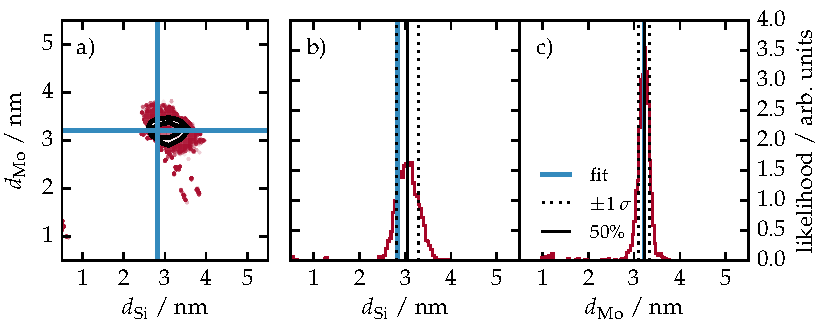
\includegraphics{img/Mo_Si_C_d_Mo_vs_d_Si}
\caption{Results of the maximum likelihood estimation obtained via the \gls{mcmc} procedure similar to Fig.~\ref{ch_spec:fig_ptb17_MCMC_d_Mo_vs_d_Si} but for the combination of \gls{euv} and \gls{xrr} data. a) Two dimensional projection of the likelihood distribution for the parameter pair $d_\text{Si}$ and $d_\text{Mo}$. The projection was obtained by marginalizing over all other parameters of the model. The black contours indicate the areas for one and two standard deviations (one and two sigma contours). The blue lines in all three sub-figures indicate the best parameter set found with the \gls{pso} method. b) One dimensional projection of the likelihood distribution for the silicon layer thickness $d_\text{Si}$. The solid black line marks the center position ($50\%$ percentile) of the distribution. The dotted lines are the limits of one standard deviation. c) The one dimensional distribution similarly to b) for the molybdenum layer thickness.}
\label{ch_spec:fig_Mo_Si_C_d_Mo_vs_d_Si}
\end{figure*}
In comparison to the analysis based on only \gls{euv} data for the Mo/B$_4$C/Si/C in Fig.~\ref{ch_spec:fig_ptb17_MCMC_d_Mo_vs_d_Si}, the inclusion of additional \gls{xrr} measurements lead to significantly smaller confidence intervals and thus higher accuracy of the reconstruction, although the two systems have a limited comparability due their different layer layouts. The method of combining the analysis of two datasets of \gls{euv} and \gls{xrr} measurements has been previously applied by others \cite{yakunin_combined_2014}, which have come to the same result of a significantly improved model reconstruction. Each of the methods does provide different sensitivity for the different model parameters. As an example, \gls{euv} measurements are sensitive to the Mo and Si layer thicknesses due to the large optical contrast in that spectral range. On the other hand, high accuracy can be expected from the \gls{xrr} measurements with respect to the period thickness parameter $D$.

In a second step, another \gls{mcmc} optimization was performed on a reduced parameter set, fixing the determined molybdenum layer thickness to its optimal value, i.e.~the $50\%$ percentile of its distribution. Finally, the layer thicknesses of the C barrier layer and the MoSi$_2$ interdiffusion layer were fixed to their nominal values of $d_C = d_{\text{MoSi}_2} = 0.5 $ nm. Due to the broad distribution result for the likelihoods of those parameters, this comes without a limitation of the generality for this analysis, since any value is valid within the predefined boundaries. Additionally, this ensures comparability of the models for all samples without constraining the applicability of the model with respect to the data available.

\begin{figure}[htbp]
\centering
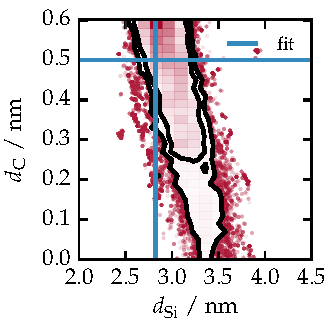
\includegraphics{img/Mo_Si_C_correlation_Si_C}
\caption{Two-dimensional likelihood distribution indicating the correlation of silicon and carbon layer thickness. The distribution was obtained by marginalizing over all remaining parameters of the model. The blue lines indicate the fit obtained through the two-step \gls{mcmc} optimization procedure (see main text).}
\label{ch_spec:fig_Mo_Si_C_correlation_Si_C}
\end{figure}
The results of the second \gls{mcmc} procedure of the restricted model yield the remaining values for the model parameters by obtaining the globally best solution found. The final result is indicated by the blue solid lines in Fig.~\ref{ch_spec:fig_Mo_Si_C_d_Mo_vs_d_Si}. Due to the choice to restrict the model to a buffer layer thickness of $d_\text{C} = \nm{0.5}$, we find the optimal solution for the silicon layer thickness at the limit of one standard deviation in Fig.~\ref{ch_spec:fig_Mo_Si_C_d_Mo_vs_d_Si}b. The distributions shown represent the \gls{mcmc} results of the unrestricted model, where the silicon and carbon layer thicknesses are strongly correlated as shown in Fig.~\ref{ch_spec:fig_Mo_Si_C_correlation_Si_C}. By fixing the carbon layer thickness to its nominal value, this correlation is resolved and the corresponding silicon layer thickness is well within the interval of one standard deviation as indicated through the solid black contours in Fig.~\ref{ch_spec:fig_Mo_Si_C_correlation_Si_C}.

\subsection{Optimization results}
The theoretical reflectivity curves calculated from the optimal model parameters for the unpolished sample with $d_\text{Mo}^\text{nom} = \nm{3.05}$ are shown in Fig.~\ref{ch_spec:fig_EUV_XRR_combined}. Overall, a very good agreement of the two experiments with the theoretical curve are obtained.
\begin{figure}[htbp]
\centering
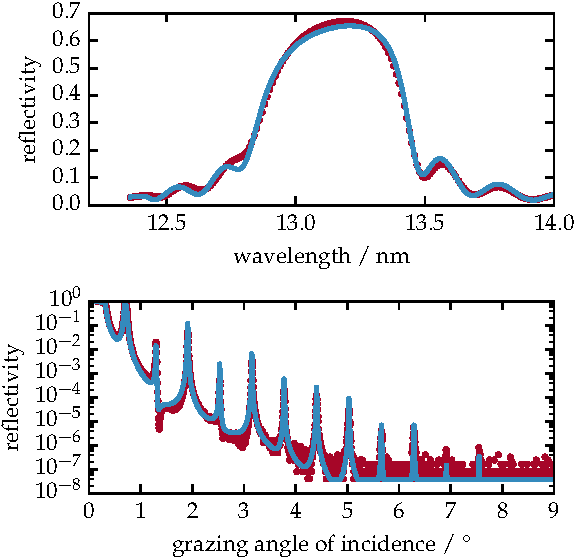
\includegraphics{img/PS5657}
\caption{Experimental data in comparison with the theoretical curves calculated with the model parameters obtained from the combined analysis of \gls{euv} and \gls{xrr} data. The data shown here was measured on the unpolished sample with nominal molybdenum thickness of $d_\text{Mo}^\text{nom} = \nm{3.05}$.}
\label{ch_spec:fig_EUV_XRR_combined}
\end{figure}
The full list for all molybdenum layer thicknesses for all samples and the respective confidence intervals in comparison to their nominal layer thickness are given in table~\ref{ch_spec:tbl_mo_si_thickness_mcmc_result}.
\begin{table}[htbp]
\centering
\caption{List of nominal molybdenum layer thicknesses in the two sample sets. Both sets were fabricated with a equidistant increase in thickness from \nm{1.70} to \nm{3.05} with 9 unpolished and 10 polished samples.}
\label{ch_spec:tbl_mo_si_thickness_mcmc_result}
\begin{tabular}{@{}lll@{}}
\toprule
nom.~$d_\text{Mo}$ / nm & EUV \& XRR &EUV \& XRR\\ 
&(unpolished) & (polished) \\
\midrule
$1.70$ &$1.81({-0.12}/{+0.24})$  &$1.77({-0.22}/{+0.19})$ \\
$1.85$ &$1.98({-0.15}/{+0.14})$  &$1.91({-0.12}/{+0.17})$ \\
$2.00$ &$2.08({-0.11}/{+0.22})$  &$2.29({-0.28}/{+0.13})$ \\
$2.15$ &$2.31({-0.22}/{+0.21})$  &$2.45({-0.43}/{+0.06})$ \\
$2.30$ &$2.43({-0.09}/{+0.16})$   &$2.60({-0.12}/{+0.14})$ \\
$2.45$ &$2.68({-0.13}/{+0.16})$  &$2.58({-0.21}/{+0.15})$ \\
$2.60$ &$2.91({-0.17}/{+0.12})$ &$2.87({-0.22}/{+0.12})$ \\
$2.75$ &$3.02({-0.15}/{+0.15})$  &$3.03({-0.16}/{+0.14})$ \\
$2.90$ &$3.22({-0.13}/{+0.11})$ &$3.15({-0.13}/{+0.13})$ \\
$3.05$ &-  & $3.47({-0.19}/{+0.13})$ \\
 \bottomrule
\end{tabular}
\end{table}

The optimal parameters for the molybdenum layer thickness $d_\text{Mo}$ and the period thickness $D$ found for both sample sets in the two-step \gls{mcmc} analysis are shown in Fig.~\ref{ch_spec:fig_MoSi_fitted_mo_and_fitted_D}.
\begin{figure*}[htbp]
\centering
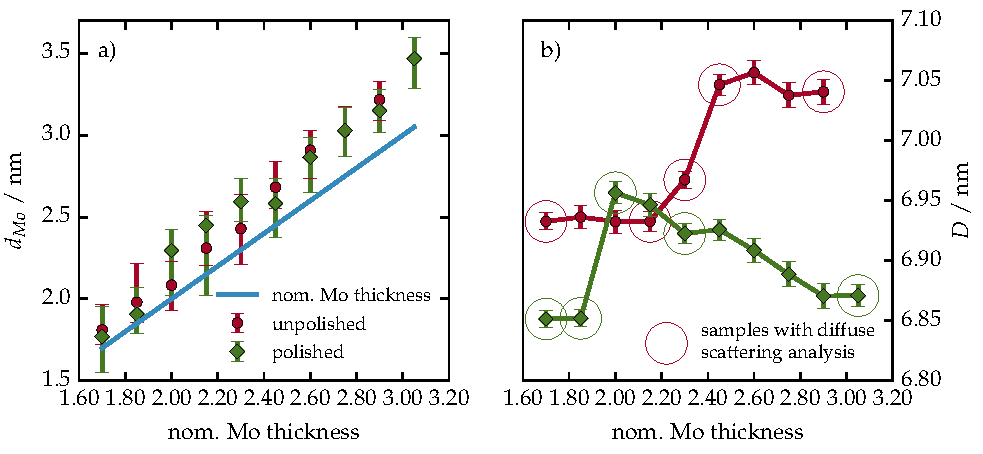
\includegraphics[width=\textwidth]{img/fitted_mo_and_fitted_D}
\caption{a) Fitted Mo thickness values for both sample sets resulting from the MCMC analysis (see text). The nominal Mo layer thickness is shown in comparison in good agreement with the obtained thicknesses. b) Fitted total period thickness $D$ for both sample sets. For both sample sets, clear jumps can be observed at approx.~$d^\text{nom}_\text{Mo} =2.00$ nm and $d^\text{nom}_\text{Mo} =2.38$ nm, respectively, which is attributed to the crystallization threshold (see text). The marked (circle) samples were measured and analyzed with respect to the diffuse scattering.}
\label{ch_spec:fig_MoSi_fitted_mo_and_fitted_D}
\end{figure*}
The confidence intervals shown in Fig.~\ref{ch_spec:fig_MoSi_fitted_mo_and_fitted_D}a are one standard deviation of the likelihood determined for the Mo layer thickness by the first-step MCMC procedure, i.e.~for the unresticted model with the parameter limits as listed in table~\ref{ch_spec:tbl_mo_si_c_multilayer_parameters}. The results show the desired linear increase in molybdenum layer thickness, however at a systematically higher thickness than the nominal values. A possible cause for that observation, consistent with the model reconstruction results, is the possible interdiffusion of the molybdenum layer with the silicon and carbon during deposition. This would reduce the relative density of the molybdenum layer. The reconstruction results for all samples indeed show systematically reduced density values of $\rho_\text{Mo} \approx 90\%$ w.r.t.~the Mo bulk density. It is reasonable to assume, that the magnetron sputtered Mo layer causes interdiffusion at the boundaries which in turn leads to density reduced layers. Thus, the nominal amount of deposited molybdenum leads to higher thicknesses than desired. In Fig.~\ref{ch_spec:fig_MoSi_fitted_mo_and_fitted_D}b the fitted period thicknesses $D$ are shown in dependency of the fitted molybdenum thicknesses.

For both sets, distinct jumps can be observed between $d_\text{Mo}\approx\nm{1.9}$ and $d_\text{Mo}\approx\nm{2.3}$ for the polished samples and between $d_\text{Mo}\approx\nm{2.3}$ and $d_\text{Mo}\approx\nm{2.7}$ for the unpolished set. To better understand this observation, Fig.~\ref{ch_spec:fig_EUV_peak_refl} shows the maximum peak reflectance of all EUV measurements also as a function of the reconstructed Mo layer thickness.
\begin{figure}[htbp]
\centering
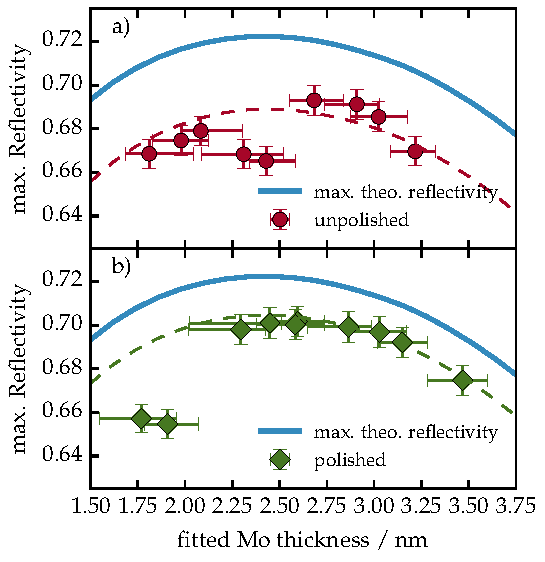
\includegraphics[width=0.6\textwidth]{img/MoSi_EUV_peak}
\caption{Peak reflectance values for each sample obtained from the \gls{euv} measurements for the unpolished sample set (a) and the polished sample set (b). The maximum theoretical reflectance is shown in both subfigures for a perfect (no roughness or interdiffusion) layer system with the same specifications as the samples.}
\label{ch_spec:fig_EUV_peak_refl}
\end{figure}
The identical blue solid line in both subfigures indicates the maximum peak reflectance attainable for a perfect multilayer system with the respective Mo layer thickness without any interdiffusion or roughness. For the calculation a carbon capping layer of $d_\text{C(cap)} = 2.0$ nm and a relative density of $\rho_\text{C(cap)} = 0.5$ and a silicon dioxide layer of $d_\text{SiO$_2$} = 2.0$ was considered. The dashed curves in both figures show the expected maximum peak reflectance values for the two sample systems calculated by adding the respective roughness/interdiffusion to the model and varying the molybdenum thickness accordingly. In both cases, a significant dip with respect to the expected value can be observed starting at thicknesses of $d_\text{Mo} = 2.31({-0.22}/{+0.21})$ nm for the unpolished samples in Fig.~\ref{ch_spec:fig_EUV_peak_refl}a and at $d_\text{Mo} = 1.77({-0.22}/{+0.19})$ nm for the polished samples in Fig.~\ref{ch_spec:fig_EUV_peak_refl}b. We attribute this significantly diminished peak reflectance to the process of crystallization as the most likely cause. These values are consistent with the increase observed in the period thickness for both cases. However, the jump in the period thickness value with the increasing molybdenum layer thickness is observed one (in case of the unpolished samples) to two data points (in case of the polished samples) after the first dip in peak reflectance. Possibly, the deposition is affected by the crystallization threshold causing the increase in period thickness. The values measured here for the dip in peak reflectance is in agreement with earlier observation of molybdenum crystallization in literature \cite{bajt_investigation_2001} for the unpolished sample set. The polishing process shifts that threshold to lower thicknesses by approximately \nm{0.2} to \nm{0.3}.

For a deeper investigation of the interface morphology during the presumed crystallization threshold, \gls{euv} diffuse scattering experiments have been conducted for selected samples of the respective set. The selection is marked with open circles in Fig.~\ref{ch_spec:fig_MoSi_fitted_mo_and_fitted_D}. To gain a deeper understanding of the reflectivity dip and the period increase, the samples in vicinity of this feature in the Fig.~\ref{ch_spec:fig_EUV_peak_refl} and Fig.~\ref{ch_spec:fig_MoSi_fitted_mo_and_fitted_D} were investigated in comparison to reference samples above and below the threshold. This analysis is the topic of chapter~\ref{ch_diff} of this thesis and described and discussed in detail there based on the model parameters obtained here.

 





\section{Analysis of Cr/Sc Multilayers with Sub-nanometer Layer Thickness}
In the previous sections we have characterized multilayer systems specifically designed to reflect radiation in the \gls{euv} spectral range from \nm{12.5} to \nm{14.0} wavelength. There, the three to four layer systems per period with period thicknesses of $D\approx\nm{7}$ were used to achieve constructive interference at the desired reflection angles. We shall now expand the analysis to a different system. Multilayer mirrors designed to reflect radiation in the spectral range between \nm{2.2} and \nm{4.4} wavelength, the so called \emph{water window}. Those systems share the basic principle of a one-dimensional Bragg crystal with the Mo/Si multilayer stacks from the previous sections, but differ in the selection of materials. The intrinsic relationship between spectral range and period thickness to achieve constructive interference, requires period thicknesses of $D\approx \nm{1.5}$ for this case and higher period replication.


The system we focus on in the rest of this chapter is composed out of a bilayer stack of chromium (Cr) and scandium (Sc). A detailed description of the sample preparation process and the choice of the layer materials can be found in Ch.~\ref{ch_exp}, Sec.~\ref{ch_exp:sec_multilayer_design}. The sample is optimized to reflect radiation of $\lambda = \nm{3.14}$ at an angle of incidence of $\alpha_i = \SI{1.5}{\degree}$. Its periodicity is $N=400$ bilayer periods, where the last period has a larger Cr capping layer thickness. The model of the sample is shown in Fig.~\ref{ch_spec:fig_Cr_Sc_model}.
\begin{figure}[htbp]
    \def\svgwidth{0.7\textwidth}
    \fontfamily{fds}\selectfont\footnotesize
    \import{svg/}{cr_sc_model.pdf_tex}
    \caption{Model of the multilayer stack including the substrate and the capping layers. The periodic part is enclosed between the dashed lines with four layers in each period repeated $N=64$ times. The capping period does not include an interdiffusion layer but has a natural SiO$_2$ layer.}
    \label{ch_spec:fig_Cr_Sc_model}
\end{figure}
The small period thickness of only $D\approx\nm{1.5}$ for this type of sample yields individual layer thicknesses in the sub-nanometer regime, for a bilayer period with approximately equal individual layer thicknesses. This is a significant difference to the Mo/Si systems treated in the beginning of this chapter, where the molybedum and silicon layers were well above $>\nm{1.7}$, even in the smallest case existed. The buffer and interdiffusion layers, which nominally have thicknesses in the same order of magnitude as expected for the Cr/Sc system, could not be characterized based on the methods employed above. We shall therefore first compare the results obtained with an approach similar to the methods in the previous sections to establish a limit to the applicability of discrete layer models.

\subsection{Reconstruction with a discrete layer model approach} \label{ch_spec:sec_CrSc_resconstrution_binary}
In analogy to Sec.~\ref{ch_spec:sec_mo_si_c}, we seek to reconstruct the individual layer thicknesses based on experimental data. For this we construct a discrete layer model as illustrated in Fig.~\ref{ch_spec:fig_Cr_Sc_model} in analogy to the procedure applied for the Mo/Si multilayer systems. The parameters of this discrete layer model are listed in table~\ref{ch_spec:tbl_cr_sc_binary_parameters} together with the upper and lower bound for the particle swarm optimization procedure.
\begin{table*}[htbp]
\centering
\caption{Parametrization of the Cr/Sc binary multilayer model.}
\label{ch_spec:tbl_cr_sc_binary_parameters}
\begin{tabular}{@{}llll@{}}
\toprule
Parameter & Definition & Lower bound & Upper bound\\ \midrule
$d_\text{Cr}$ / nm & Cr layer thickness & $0.0$& $1.5$\\ 
$d_\text{Sc}$ / nm & Sc layer thickness& $0.0$& $1.5$\\ 
$\sigma$ / nm & N\'{e}vot-Croce parameter& $0.0$& $0.5$\\ 
&(identical for all interfaces)&&\\
$\rho_\text{Cr}$ &Cr density w.r.t.~bulk density & $0.5$& $1.0$\\ 
$\rho_\text{SC}$ &Sc density w.r.t.~bulk density& $0.5$& $1.0$\\ 
\midrule
\multicolumn{4}{c}{Capping layer}\\
\midrule
$d_\text{C (cap)}$ / nm & C capping layer thickness & $0.0$&$1.0$ \\ 
$d_\text{CrO (cap)}$ / nm & SiO$_2$ capping layer thickness & $0.0$&$1.5$ \\ 
$d_\text{Cr (cap)}$ / nm & SiO$_2$ capping layer thickness & $0.0$&$3.0$ \\ 
$\rho_\text{C (cap)}$ &C density w.r.t.~bulk density& $0.0$& $1.0$\\ 
$\rho_\text{CrO (cap)}$& CrO density w.r.t.~bulk density& $0.0$& $1.0$\\
$\rho_\text{Cr (cap)}$& Cr (cap) density w.r.t.~bulk density & $0.5$& $1.0$  \\
 \bottomrule
\end{tabular}
\end{table*}

The reflectivity of the sample in the water window spectral range from \nm{3.12} to \nm{3.16} was measured at the \gls{sx700} beamline at \gls{bessy}. The angle of incidence was $\alpha_i=\SI{1.5}{\degree}$ (corresponding to a grazing angle of incidence of $\alpha_i^\text{GI} = \SI{88.5}{\degree}$), which corresponds to the design goal for this mirror prototype. In addition, similar to the Mo/Si samples, a \gls{xrr} measurement was 
conducted in the DESY laboratory using a laboratory-based X-ray diffractometer 
(X'Pert PRO MRD, Panalytical). The diffractometer is equipped with a high-resolution goniometer and uses Cu-K$_\alpha$ radiation as a source. The \gls{xrr} intensities were recorded using a PIXcel counting detector. The dynamic range achieved in the measurements 
extended down to a reflectance of $10^{-6}$ for grazing angles of incidence of 
$\alpha_i=0^\circ$ to $\alpha_i=3^\circ$.

Both measurement curves are shown together in Fig.~\ref{ch_spec:fig_CrSc_EUV_XRR_data}.
\begin{figure}[htbp]
  \centering
  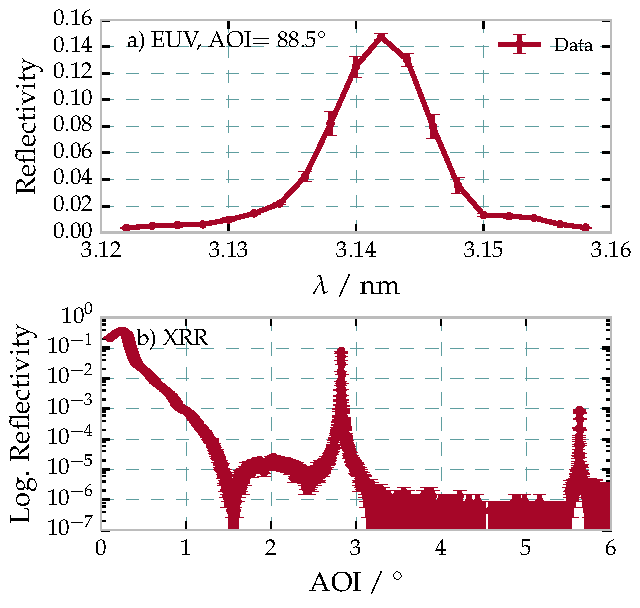
\includegraphics[width=0.6\textwidth]{img/CrSc_EUV_XRR_data}
  \caption{\Gls{euv} and \gls{xrr} data recorded for the Cr/Sc sample system. a) The \gls{euv} curve was obtained at an angle of incidence $\alpha_i=\SI{1.5}{\degree}$. b) The \gls{xrr} curve was recorded using a Cu-K$_\alpha$ source with a photon energy of $E_\text{ph}=\ev{8048}$.}
  \label{ch_spec:fig_CrSc_EUV_XRR_data}
\end{figure}
Due to the short period of the multilayer sample, only two Bragg peaks could be observed in this angular range in the \gls{xrr} curve. All expected higher order peaks were below the detection threshold of $10^{-6}$ in reflected intensity. The dominating experimental uncertainty was the inhomogenity of the sample stack across the sample area. The given uncertainty values for each of the measurement points were estimated, by measuring the peak reflectance of the \gls{euv} reflectivity curve on positions marking a cross of \mm{2} by \mm{2} in the sample center. This data was compared to theoretical expectance value based on a \gls{pso} fit of the discrete layer model above (for details of the optimization results see below). From this a drift of the period thickness of $D=\SI{2}{\pico\meter}$ was obtained and uncertainties were calculated as the difference of two theoretical curves attaining the maximum and minimum $D$ values. Similarly, uncertainties for the \gls{xrr} curve was calculated by simulating theoretical curves based on the same period drifts.

In comparison, the most remarkable difference with respect to the Mo/Si mirrors is the significantly reduced peak reflectance of the \gls{euv} curve in Fig.~\ref{ch_spec:fig_CrSc_EUV_XRR_data}a compared to the curves in Fig.~\ref{ch_spec:fig_ptb17_reflectance_AOI_15} and Fig.~\ref{ch_spec:fig_EUV_reflectivity_unpolished_and_polished_with_peak_refl}c. The maximum experimental value attained is only approximately $R_\text{max} \approx 15\%$ while it is up to $R_\text{max} \approx \SI{70}{\percent}$ for the Mo/Si systems. The reasons for this are the different spectral range and the material properties at the water window wavelengths.

To better illustrate the differences to the Mo/Si systems, we have conducted an 
analysis based on the discrete layer model of a Cr/Sc multilayer as described above. The particle swarm optimization was done based on the EUV data shown in Fig.~\ref{ch_spec:fig_CrSc_EUV_XRR_data}a and the parameters and limits listed in table~\ref{ch_spec:tbl_cr_sc_binary_parameters}. The resulting parameters are listed in table~\ref{ch_spec:tbl_cr_sc_binary_pso_results}.
\begin{table}[htbp]
\centering
\caption{\gls{pso} fit results for the discrete layer Cr/Sc multilayer model.}
\label{ch_spec:tbl_cr_sc_binary_pso_results}
\begin{tabular}{@{}ll@{}}
\toprule
Parameter &  \gls{pso} result\\ \midrule
$d_\text{Cr}$ / nm &  $0.8224$\\ 
$d_\text{Sc}$ / nm &  $0.7510$\\ 
$\sigma$ / nm &  $0.375$\\ 
$\rho_\text{Cr}$  & $0.876$\\ 
$\rho_\text{Sc}$ & $0.957$\\ 
\midrule
\multicolumn{2}{c}{Capping layer}\\
\midrule
$d_\text{C (cap)}$ / nm  & $0.462$ \\ 
$d_\text{CrO (cap)}$ / nm  & $1.143$ \\ 
$d_\text{Cr (cap)}$ / nm  & $2.322$ \\ 
$\rho_\text{C (cap)}$ & $0.502$\\ 
$\rho_\text{CrO (cap)}$& $0.618$\\
$\rho_\text{Cr (cap)}$ & $0.851$\\
 \bottomrule
\end{tabular}
\end{table}
The capping layer results were obtained in a combined \gls{pso} analysis based on the \gls{euv} and \gls{xrr} data excluding the areas of the Bragg peaks. This grazing incidence reflectivity data has a very high sensitivity for the top surface layers, which can not be deducted from an \gls{euv} curve alone as demonstrated in Sec.~\ref{ch_spec:sec_reconstruction_PTB17}.

The theoretical curve obtained from the \gls{pso} procedure is shown in Fig.~\ref{ch_spec:fig_CrSc_binary_fit_vs_max_refl} in direct comparison with the theoretically achievable maximum reflectivity curve.
\begin{figure}[htbp]
  \centering
  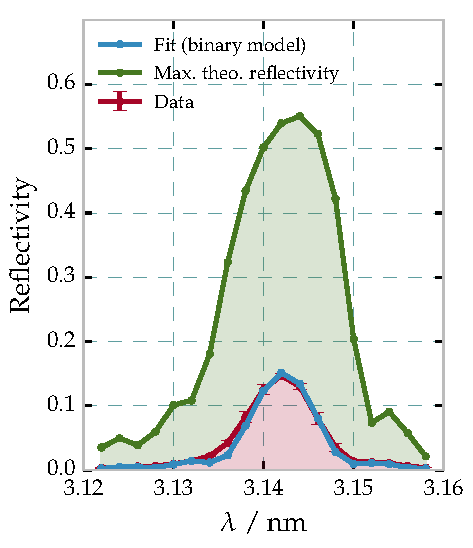
\includegraphics[width=0.45\textwidth]{img/CrSc_binary_fit_vs_max_refl}
  \caption{Fitted experimental EUV reflectance curves across the wavelength 
of the radiation impinging at $\alpha_i=1.5^\circ$ from normal, based on the binary 
model. The green curve shows the maximum theoretical reflectance assuming a perfect multilayer system without roughness or interdiffusion.}
  \label{ch_spec:fig_CrSc_binary_fit_vs_max_refl}
\end{figure}
The latter was obtained by calculating the resulting reflectivity based on the parameter results in table~\ref{ch_spec:tbl_cr_sc_binary_pso_results}, but without any roughness or interdiffusion, i.e.~by requiring $\sigma \equiv 0.0$. The Sc 
to Cr ratio was found to be $\Gamma_\text{Sc}= d_\text{Sc}/d_\text{Cr} = 0.48$ with a \gls{rms} value of $\sigma=0.385$ nm for the N\'{e}vot-Croce factor. While the EUV reflectance curve shows excellent agreement with the measured data, there is a significant offset to the theoretically achievable maximum reflectance. For the particular model derived above, theoretical reflectance values of $R_\text{max} > \SI{50}{\percent}$ are possible. This large difference, especially compared to Mo/Si systems which are very close to the theoretically achievable maximum reflectance (cf.~Fig.~\ref{ch_spec:fig_EUV_peak_refl}), hints at strong roughness or intermixing of the two materials. To verify the applicability of the discrete (binary) layer model used here, the calculated curves for both experiments, the \gls{euv} and \gls{xrr} curve, are shown together in Fig.~\ref{ch_spec:fig_CrSc_binary_model_EUV_vs_XRR}.
\begin{figure*}[htbp]
  \centering
  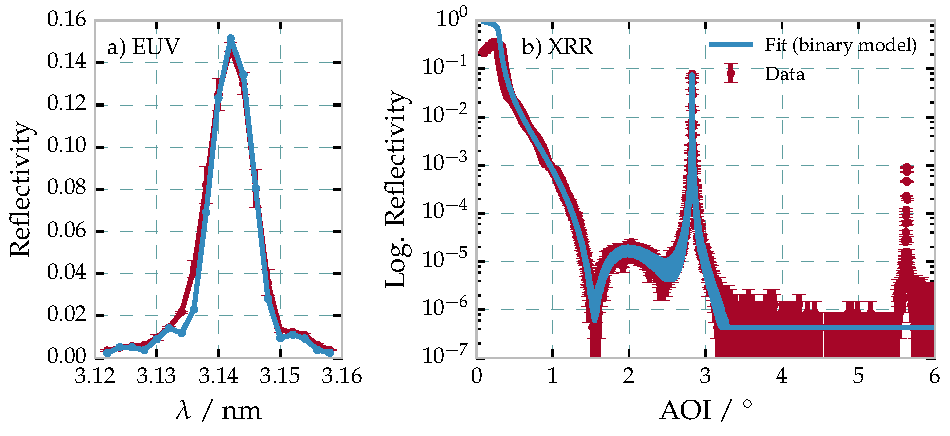
\includegraphics[width=\textwidth]{img/CrSc_binary_model_EUV_vs_XRR}
  \caption{a) Measured \gls{euv} reflectivity curve for the near-normal angle of incidence of $\alpha_i=\SI{1.5}{\degree}$ together with the theoretical curve based on the \gls{pso} optimized binary multilayer model. b) Measured and calculated \gls{xrr} curves for the same sample and model parameters at grazing angles of incidence using radiation at the Cu-K$_\alpha$ wavelength. A clear mismatch of the theoretical curve and the measured data can be observed for the second Bragg peak between $\alpha_i^\text{GI} = \SI{5.0}{\degree}$ and $\alpha_i^\text{GI} = \SI{6.0}{\degree}$.}
  \label{ch_spec:fig_CrSc_binary_model_EUV_vs_XRR}
\end{figure*}

Again, the \gls{euv} data is matched excellently, while in the case of the \gls{xrr} measurement the first Bragg peak is found to be matched by the model also in the X-ray regime. However, the second Bragg resonance, clearly visible with a peak reflectance value of approximately $10^{-3}$ is not represented by the model at all. A fully
combined analysis similarly to the approach in Sec.~\ref{ch_spec:sec_mo_si_c} could not yield a consistent result. The \gls{rms} value for $\sigma$ required to reduce the theoretical EUV reflectance down to the measured 
level could not be brought into agreement with the second Bragg peaks in the \gls{xrr} curve. In a strictly binary model like this one with a layer thickness ratio of 
$\Gamma_\text{Sc}\approx 0.5$, the second Bragg peak is additionally suppressed 
due to symmetry reasons. Thus, there is a clear mismatch of the model reconstruction and the experimental observations, mostly due to the complementary data delivered through the measurement of the second Bragg peak of the \gls{xrr} curve. This is a strong indicator, that the simple model as defined above does not suffice to describe the physical situation of the sample. Therefore, a more elaborate model is required introducing additional parameters to account for the increased complexity of the samples layer properties compared to the Mo/Si sample systems above.

\subsection{Extending The Model to Graded Interfaces and Interdiffusion} \label{ch_spec:sec_CrSc_gradual_model}
The physical situation of Cr/Sc multilayer systems with individual layer thicknesses in the sub-nanometer regime is significantly different than in comparably large thicknesses of several nanometers such as in the Mo/Si case of the two preceding sections. It is well known \cite{prasciolu_thermal_2014}, that magnetron sputtered Cr and Sc multilayer systems, similarly to the Mo/Si systems, suffer from imperfect interfaces. The main reason for that is interdiffusion of the two materials into each other. In addition, roughness at the interfaces exists and further diminishes an ideal chemically abrupt transition from one material to the next. Due to the small layer thicknesses required to achieve the first Bragg resonance upon near-normal incidence with radiation of $\lambda=\nm{3.14}$, roughness and interdiffusion may occur over an interdiffusion zone as large as the total layer thickness itself. The results from the specular \gls{euv} and \gls{xrr} measurements shown above, clearly demonstrate that a binary model with only a N\'{e}vot-Croce damping parameter $\sigma$ due not provide an accurate model for the physical reality. Instead, a more complex model is required. Here, we define a periodic model, repeated in units of one bilayer period, to account for possible interdiffusion gradients and intermixing between the two materials in the stack. The symmetry of two identically thick layers within one period in the simple model above leads to a suppression of the second order Bragg peak. Nevertheless, physically this symmetry effect can be broken by accounting for interdiffusion zones with different thicknesses, depending on whether Cr was deposited on Sc or vice versa. Thereby, the second Bragg peak is no longer suppressed even though both layers have the same thickness if the interdiffusion zones are asymmetric. Physical causality further dictates, that the two layers intermix gradually. The model, which we use to reconstruct the Cr/Sc multliayer sample measured above is illustrated in Fig.~\ref{ch_spec:fig_CrScModel} in direct comparison to the simple model used before.
\begin{figure*}[htb]
    \def\svgwidth{\textwidth}
    \import{svg/}{CrSc_model.pdf_tex}
    \caption[Binary and gradual Cr/Sc multilayer models.]{a) Binary Cr/Sc multilayer model with total period thickness $D$ and 
the individual layer thicknesses $d_\text{Sc}$ and $d_\text{Cr}$. b) Model with 
explicit gradual interfaces following a sinusoidal profile. The ideal interface 
profile is approximated through discrete sublayers as indicated in red, forming 
the actual gradual interface profile entering the electric field calculations. 
The thickness of the interdiffusion zones can differ for the top and bottom 
interface in each period. Their total thicknesses are given by $s_\text{Sc}$ 
and $s_\text{Cr}$. The effective index of refraction for both layers is given 
by $\tilde{n}_\text{Sc}$ and $\tilde{n}_\text{Cr}$, respectively.}
    \label{ch_spec:fig_CrScModel}
\end{figure*}
The interdiffsion zones are modeled following a sinosodial profile, which represents a smooth transition from the refractive index of the Cr layer to the Sc layer and vice versa. The thickness of those zones is given by the parameters $s_\text{Sc}$ and $s_\text{Cr}$. For the calculation of the electromagnetic fields inside the stack, the interface region is sampled with a fixed number of equally spaced points in $z$-direction, effectively creating a region of thin sublayers with a gradually changing index of refraction (illustrated by the red steped function in Fig.~\ref{ch_spec:fig_CrScModel}). To take into account intermixing extending across the full period, we introduced an intermixing parameter $\eta$. The effective indices of refraction of the individual Cr and Sc layers are then given through
\begin{align}
\tilde{n}_\text{Cr} &=(\eta/2) n_\text{Sc} + (1-\eta/2) n_\text{Cr} \text{,} 
\nonumber\\
\tilde{n}_\text{Sc} &=(1-\eta/2) n_\text{Sc} + (\eta/2) n_\text{Cr} \text{,} 
\label{eqn:effective_n} \\
&\text{for} \quad \eta \in [0,1] \text{,}\nonumber
\end{align}
where $n_\text{Cr}$ and $n_\text{Sc}$ are the tabulated values \cite{henke_x-ray_1993} 
with densities $\rho_\text{Cr}$ and $\rho_\text{Sc}$.

With the definition of the model as outlined above, natural restrictions arise for the parameters. As an example, the interdiffusion zone region can not extend across half of the thickness of the original layers total thickness described by the parameter $d_\text{Cr}$ or $d_\text{Sc}$, respectively. Instead, the intermixing parameter would have to be increased to account for that situation. The model is therefore parameterized according to the list of effective parameters given in table~\ref{ch_spec:tbl_CrSc_gradual_parametrization} together with their allowed ranges for the optimization procedure in analogy to the analysis conducted in the previous sections. The range limits arise either from physical plausibility or are intrinsic properties of the parameter definition.
\begin{table*}[htbp]
\centering
\caption{Multilayer parametrization and parameter limits}
\label{ch_spec:tbl_CrSc_gradual_parametrization}
\begin{tabular}{@{}llll@{}}
\toprule
Parameter & Definition & Lower bound & Upper bound\\ \midrule
$D$ / nm & $= d_\text{Sc} + d_\text{Cr}$ & 1.5&1.6 \\ 
$\Gamma_{Sc}$ & $= d_\text{Sc} / D$&0.0 &1.0 \\ 
$s_d$ / nm&$=s_\text{Sc} + s_\text{Cr}$&0.0 & 1.6\\ 
$\Gamma_s$ &$= s_\text{Sc} / s_d$& 0.0& 1.0\\ 
$\eta$ &layer intermixing& 0.0& 1.0\\ 
$\sigma_r$ / nm & r.m.s.~roughness& 0.0& 0.5\\ 
$\rho_{Sc}$ &Sc density w.r.t.~bulk density & 0.5& 1.0\\ 
$\rho_{Cr}$ &Cr density w.r.t.~bulk density& 0.5& 1.0\\ 
 \bottomrule
\end{tabular}
\end{table*}
Here, $D$ is the full period thickness, $d_\text{Sc}$ and $d_\text{Cr}$ are the 
nominal layer thicknesses of the Cr and Sc layers as indicated in 
Fig.~\ref{ch_spec:fig_CrScModel}, and $\rho_\text{Sc}$ and $\rho_\text{Cr}$ their 
respective densities with respect to their bulk densities 
$\tilde{\rho_\text{Sc}} = 2.989$ g/cm$^3$ and $\tilde{\rho_\text{Cr}} = 7.19$ 
g/cm$^3$ \cite{henke_x-ray_1993}. The loss of specular 
reflectance due to roughness-induced scattering is considered through the 
N\'{e}vot-Croce factor using $\sigma_\text{r}$ identical at each interface. This is necessary to account for diffusely scattered light, which is missing in the measured specularly reflected radiation but can not be attributed to contrast loss due to interdiffusion. The parameter $\Gamma_\text{Sc}$ indicates the portion of the Sc layer thickness 
with respect to the full period thickness $D$, which together uniquely define the thickness $d_\text{Cr}$; $\Gamma_\sigma$ describes the 
asymmetry of the widths of the interdiffusion zones at the Cr on Sc and Sc on Cr 
interfaces and is intrinsically limited to the interval $\Gamma_\sigma \in [0,1]$. Note that 
$s_\text{Sc}$ and $s_\text{Cr}$ are half periods of the sinus functions used to 
describe the interface profiles. Therefore the condition $s_\text{Sc} + 
s_\text{Cr} \leq D$ holds.

The discretization of the smooth interface profile in the interdiffusion zones introduces an additional numerical uncertainty through the number of discretization points $n$ required to reflect the physical situation of a smooth transition. To assert a lower limit for this number, we have evaluated the mean error introduced by coarse sampling. The most accurate experiment of the analysis within this chapter is given by the \gls{euv} reflectivity curve, which serves as a reference for this assertation through the sum of the squared uncertainty of each data point in Fig.~\ref{ch_spec:fig_CrSc_EUV_XRR_data}a, $\sum_m \tilde{\sigma}_m$. 

The numerical error of the model depending on the interface sampling through gradual sublayers was evaluated by comparing the sum of squares
\begin{align}
\chi_n &= \sum\limits_m (I^{n=100}_m - I^n_m)^2
\end{align}
of the difference of the theoretical \gls{euv} curves with increasing numbers of gradual interfaces and an ``ideal'' smooth transition represented by $100$ sublayers. The model parameters used for this analysis were obtained through a \gls{pso} optimization of the model with respect to the \gls{euv} reflectivity curve.
\begin{figure}[htbp]
  \centering
  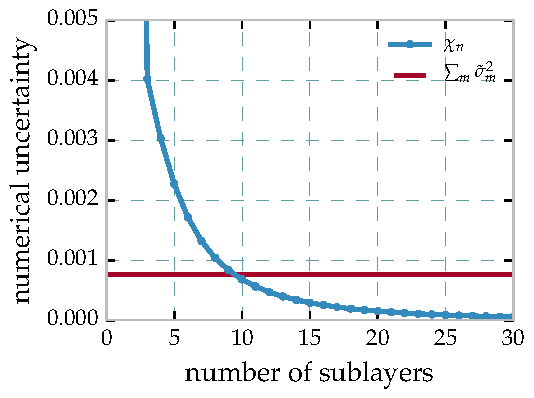
\includegraphics[width=0.45\textwidth]{img/CrSc_numerical_uncertainty_mixlayer}
  \caption{Numerical uncertainty introduced through a coarse graded layer model in comparison with the experimental uncertainty.}
  \label{ch_spec:fig_CrSc_numerical_uncertainty_mixlayer}
\end{figure}
As illustrated in Fig.~\ref{ch_spec:fig_CrSc_numerical_uncertainty_mixlayer}, the experimental uncertainty dominates at the lower limit of $n=10$ sublayers for the interface zone.
For the analysis is this chapter, and due to reasons of numerical efford required to calculate the electromagnetic field for all measurements discussed here, we use $n=15$ sublayers for all calculations. At that value, the experimental uncertainty is clearly dominant and only a marginal additional uncertainty is aquired due to insufficient sampling.

As a verification of the applicability of the model to the problem of accurately representing a physical situation that could describe the \gls{euv} and \gls{xrr} data shown in Fig.~\ref{ch_spec:fig_CrSc_EUV_XRR_data} above, we have applied the combined analysis technique for the two data sets described in Sec.~\ref{ch_spec:sec_MoSi_euv_xrr_combined} to the improved gradual model. The particle swarm optimization approach is applied to obtain a global solution for the model parameters by minimizing the functional defined in Eq.~\eqref{ch_spec:eqn_Mo_Si_C_total_chi_2}. The results found for the binary model (cf.~Fig.~\ref{ch_spec:fig_CrSc_binary_model_EUV_vs_XRR}) and the gradual model are shown in direct comparison with each other in Fig.~\ref{ch_spec:fig_CrSc_bianry_vs_gradual_model_fits}.
\begin{figure*}[htbp]
  \centering
  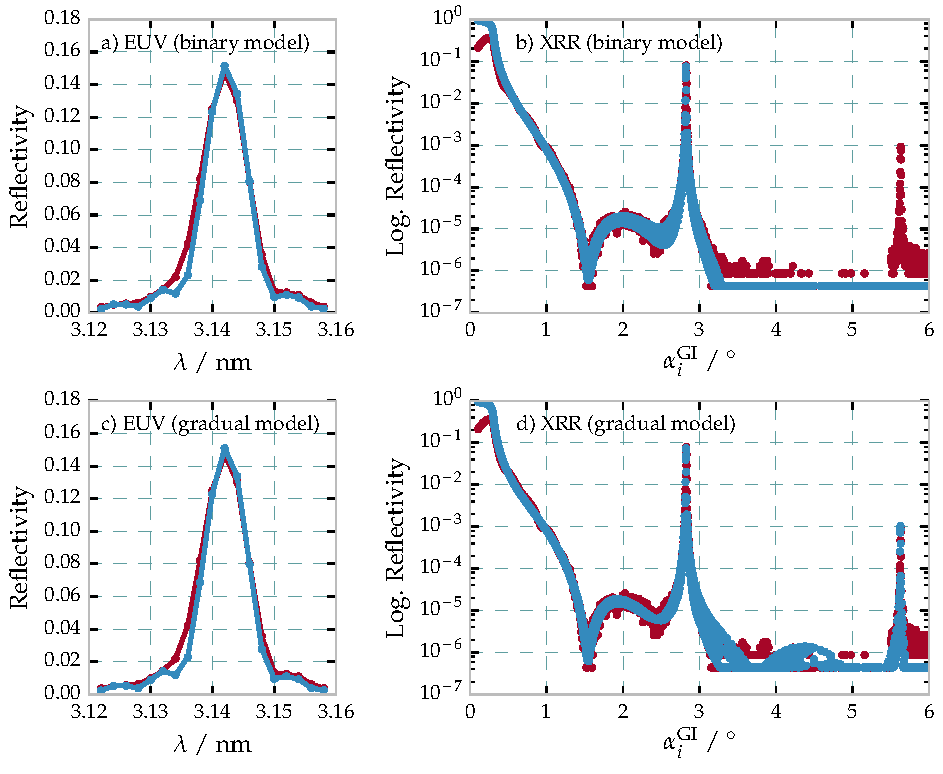
\includegraphics[width=\textwidth]{img/CrSc_bianry_vs_gradual_model_fits}
  \caption{Comparison of the reconstructions of the binary and gradual models for the \gls{euv} and \gls{xrr} data. a) Measured \gls{euv} reflectivity curve for and near-normal angle of incidence of $\alpha_i=\SI{1.5}{\degree}$ together with calculated curve of the \gls{pso}-based binary model reconstruction. b) Measured and calculated \gls{xrr} curves for the same sample and model parameters at grazing angles of incidence using radiation at the Cu-K$_\alpha$ wavelength. A clear mismatch of the theoretical curve and the measured data can be observed for the second Bragg peak between $\alpha_i^\text{GI} = \SI{5.0}{\degree}$ and $\alpha_i^\text{GI} = \SI{6.0}{\degree}$.
  c) Measured \gls{euv} reflectivity curve for and near-normal angle of incidence of $\alpha_i=\SI{1.5}{\degree}$ together with calculated curve of the \gls{pso}-based gradual model reconstruction. d) Measured and calculated \gls{xrr} curves for the same sample and model parameters at grazing angles of incidence using radiation at the Cu-K$_\alpha$ wavelength.}
  \label{ch_spec:fig_CrSc_bianry_vs_gradual_model_fits}
\end{figure*}
The \gls{euv} reflectivity curves show visually indistinguishable fits for both, the binary model as already found above and also the gradual model in Fig.~\ref{ch_spec:fig_CrSc_bianry_vs_gradual_model_fits}a and Fig.~\ref{ch_spec:fig_CrSc_bianry_vs_gradual_model_fits}c. For the binary model, we have seen the distinct mismatch with the second order Bragg peak, which is shown once again in Fig.~\ref{ch_spec:fig_CrSc_bianry_vs_gradual_model_fits}b. For the gradual interface model, we see a significant improvement of the optimized result with perfectly match in both Bragg peaks of the \gls{xrr} curve in Fig.~\ref{ch_spec:fig_CrSc_bianry_vs_gradual_model_fits}d while also maintaining an excellent agreement with the \gls{euv} curve.

Based on the example of a combined analysis of \gls{euv} and \gls{xrr} data in this section, the gradual interface model clearly provides a more accurate representation of the physical reality in the sample than the binary approach by offering a reconstruction satisfying both data sets. At the same time, the results show that a verification of the model only becomes possible by adding complementary information. In case of the example above, that information is provided through the appearance of a second Bragg peak in the \gls{xrr} curve. Thereby, the limiting case of the binary model, which is still possible for the new gradual model, can be excluded with certainty through the comparison shown in Fig.~\ref{ch_spec:fig_CrSc_bianry_vs_gradual_model_fits}. The main difference of both models is the local gradual change of the index of refraction, which attributes for the fact that both materials can intermix. More importantly, both materials can intermix differently with respect to the specific interface, i.e.~the situation where Cr is deposited on top of Sc or vice versa. A key element of obtaining a reconstruction of that particular model is thus the application of techniques, which can deliver information on the spacial distribution of the materials within one period.

At that point, it should be noted that other distortions of a perfect layer system can be imagined, which are not covered by a strictly periodic model as the one introduced above. Those include drifts of the period thickness $D$ across the stack or other systematic aperiodicities. In that case, however, a broadening of the peak or a distortion of the peaks symmetry, most prominently in the \gls{euv} curve, would be observed, which is not the case. Although situations may occur, where the aperiodicities could lead to effects compensated by tuning the parameters of the gradual interface model, this assumption would assume a more complex situation than the simple assumption of periodicity and is thus implausible.
To further strengthen that argument, we shall calculate the distortion occurring through a drift in the depostion process. This is a plausible systematic error, which could be caused by instabilities in the deposition process. Fig.~\ref{ch_spec:fig_CrSc_drift} shows the peak distortion for a drift of the total period thickness $D$ across the whole stack of $N=400$ periods by $d_\text{drift} = \nm{0.005}$ based on the model parameters for the curves in Fig.~\ref{ch_spec:fig_CrSc_bianry_vs_gradual_model_fits}c. Clearly, already this small drift would cause a distortion of the peak symmetry, which is not observed in the data and a drift thus unlikely.
\begin{figure}[htbp]
  \centering
  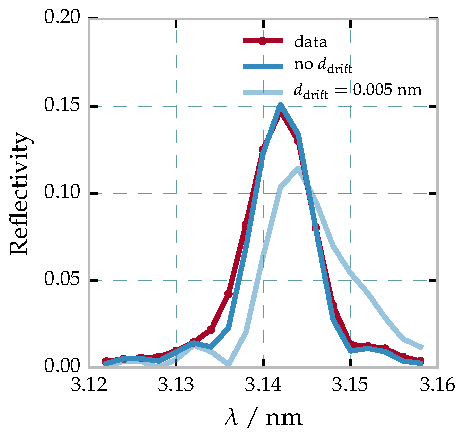
\includegraphics{img/CrSc_drift}
  \caption{\Gls{euv} peak deformation assuming a constant drift of $d_\text{drift} = \nm{0.005}$ across the total multilayer stack.}
  \label{ch_spec:fig_CrSc_drift}
\end{figure}

\subsection{Addition of Complementary Experimental Methods}
Due to the increased complexity of the model, the question arises how accurately any parameter of the model can be determined and whether correlations exist and can be resolved (cf.~Fig.~\ref{ch_spec:fig_Mo_Si_C_correlation_Si_C} as an example for correlated model parameters in case of Mo/Si multilayer systems) based on the available data and whether further analytical measurements can improve the result as this was clearly the result for the \gls{euv} and \gls{xrr} experiments shown above. For the particular case of the gradual interface model for periodic multilayer systems with sub-nanometer layer thicknesses, in total four experiments were conducted to study the applicability of each method with respect to finding a unequivocal reconstruction including confidence intervals. Only by systematically analyzing the strength and weaknesses of the employed analytic methods, a reconstruction of the model resembling the reality inside the sample becomes possible.

\subsubsection{Resonant EUV Reflectivity}
As seen for the four layer system discussed in Sec.~\ref{ch_spec:sec_reconstruction_PTB17}, confidence intervals for the individual layer thicknesses in the range below \nm{1} could not be obtained by exclusively analyzing the \gls{euv} curve. Similarly, the combined analysis of \gls{euv} and \gls{xrr} experiments in Sec.~\ref{ch_spec:sec_MoSi_euv_xrr_combined} did improve the result but still shows fairly large confidence intervals concerning the small total layer thickness in the Cr/Sc systems. For the particular system discussed here with possibly strong interdiffusion, a technique is required that yields the total amount of Sc and equivalently Cr within a single period. For that purpose, resonant reflectivity experiments in the \gls{euv} spectral range are promising. The knowledge of the optical constants are a necessary requirement for deducting quantitative information from that kind of experiment. In case of Sc, those were measured precisely for the Sc L3 and L2 absorption edges at approximately $\lambda_\text{Sc-L} \approx \nm{3.1}$ and below by \textcite{aquila_measurements_2004}. The real and imaginary parts obtained from that experiments are shown together with the respective optical constants of Cr in Fig.~\ref{ch_exp:fig_crsc_contrast} of Sec.~\ref{ch_exp:sec_multilayer_design} in  Ch.~\ref{ch_exp}. To exploit the information contained in the optical constants of Sc, angular resolved reflectivity curves across the first Bragg peak were recorded at several wavelengths across the Sc L-edge. As the Cr dispersion is changing only marginally and smoothly across that wavelength range, any change of contrast and absorption can be attributed to the Sc in the multilayer. The corresponding measurements are shown in Fig.~\ref{ch_spec:fig_CrSc_REUV_data}.
\begin{figure}[htbp]
  \centering
  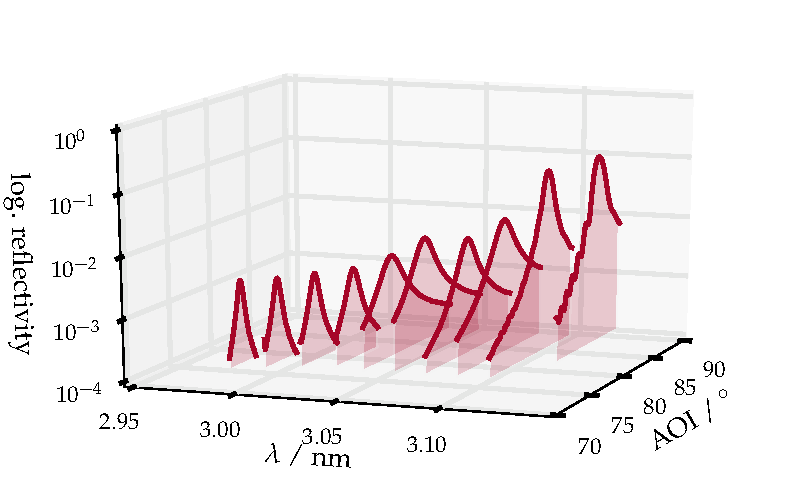
\includegraphics[width=0.7\textwidth]{img/CrSc_REUV_data}
  \caption{Measured resonant \gls{euv} reflectivity curves across the Sc L2 and L3-edge in logarithmic representation. At each equidistant photon energy point, an angular resolved reflectivity curve was recorded across the Bragg peak.}
  \label{ch_spec:fig_CrSc_REUV_data}
\end{figure}
Each reflectivity curve was recorded within the interval from $\alpha_i = \SI{2.5}{\degree}$ to $\alpha_i = \SI{19.0}{\degree}$, depending on the selected wavelength. The wavelength range was chosen between $\lambda = \nm{2.986}$ and $\lambda = \nm{3.128}$ including the Sc L2 and L3 edges. The resulting data is analyzed in analogy to the \gls{euv} reflectivity curves in Sec.~\ref{ch_spec:sec_CrSc_gradual_model} by applying the matrix algorithm on basis of the gradual layer model and the optical constants by \textcite{aquila_measurements_2004}. The experimental uncertainties taken into account for the \gls{reuv} experiment were estimated on basis of the multilayer inhomogenity deducted as described for the \gls{euv} experiment in Sec.~\ref{ch_spec:sec_CrSc_resconstrution_binary}. The details of the reconstruction based on this dataset are shown below in this section.

\subsubsection{Grazing Incidence X-ray Fluorescence}
In addition to the reconstruction of the Sc content via the \gls{reuv} experiment, spacial resolved measurements are necessary to deduct the interface profile in the gradual layer model. As discussed in Sec.~\ref{ch_spec:sec_CrSc_gradual_model}, asymmetric interface regions provide a possibility to observe a second Bragg peak in the \gls{xrr} measurement, even though both layers in the period have equal nominal thickness. To obtain information on that spacial distribution of both materials within a period, \gls{xrf} experiments exploiting the formation of a standing wave when scanning across the first Bragg peak were performed. The details of the method and how spacial sensitivity can be obtained are described in detail in Ch.~\ref{ch_theo}, Sec.~\ref{ch_theo:sec_xrf}.

The sample was measured exciting fluorescence of the Sc and Cr K-lines, which show the highest fluorescence yield for the core shell transitions. The K-edges for both materials are at energies of $E_\text{Sc-K} = \ev{4492}$ and $E_\text{Cr-K} = \ev{5989}$ \cite{elam_new_2002}. The experiment was therefore conducted at the \gls{fcm} beamline at \gls{bessy} in grazing incidence geometry at photon energies of $E_\text{ph} = \ev{5500}$ and $E_\text{ph} = \ev{6250}$, well above the respective edges as described in Ch.~\ref{ch_exp}, Sec.~\ref{ch_exp:sec_xrf_at_fcm}. Depending on which energy was used, the Bragg peak is found at grazing angles of incidence of $\alpha_i^\text{GI} \approx \SI{4.12}{\degree}$ and $\alpha_i^\text{GI} \approx \SI{3.62}{\degree}$, respectively. The measured relative fluorescence yield in the vicinity of the first Bragg peak is shown in Fig.~\ref{ch_spec:fig_CrSc_fluorescence_data} for both photon energies and materials.
\begin{figure*}[htbp]
  \centering
  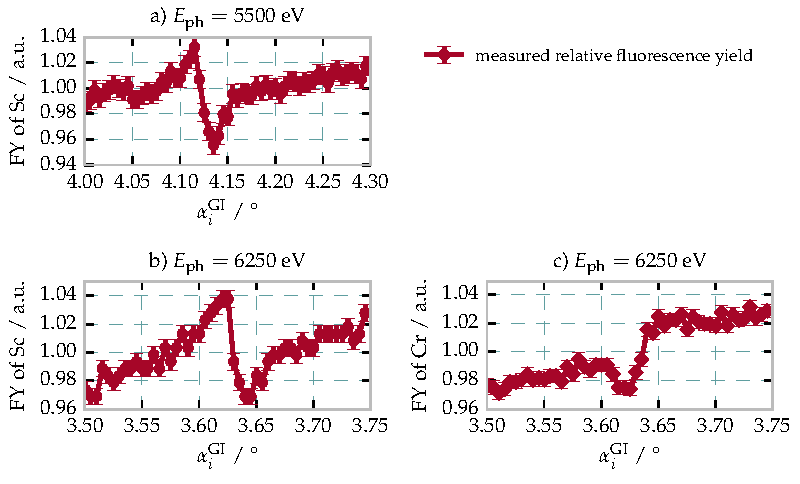
\includegraphics[width=\textwidth]{img/CrSc_fluorescence_data}
  \caption{Measured relative X-ray fluorescence curves for the Cr and Sc K-lines across the first Bragg peak. a) Relative fluorescence yield of the Sc K-line at a primary photon energy of $E_\text{ph}=\ev{5500}$. b), c) Relative fluorescence yield for both materials at an primary photon energy of $E_\text{ph} = \ev{6250}$.}
  \label{ch_spec:fig_CrSc_fluorescence_data}
\end{figure*}
Since the photon energy of $E_\text{ph} = \ev{5500}$ is below the K-edge of Cr, only data for the Sc K-fluorescence exists. In the second case, fluorescence from both materials was detected. The measurement uncertainties were estimated from the distribution of the data for regions away from the Bragg resonance.

The fluorescence curves for Cr and Sc show distinctly different behavior, of the expected curve shape (cf.~Fig.~\ref{ch_theo:fig_xrf_scheme}). For the analysis, the result at photon energies of $E_\text{ph}=\ev{5500}$ (Fig.~\ref{ch_spec:fig_CrSc_fluorescence_data}a)  was not taken into account, as the information is redundant to the result at  $E_\text{ph}=\ev{6250}$ (Fig.~\ref{ch_spec:fig_CrSc_fluorescence_data}b). As mentioned above, the theoretical description on how the relative fluorescence is calculated based on the gradual model is elaborated on in detail in Ch.~\ref{ch_exp}, Sec.~\ref{ch_exp:sec_xrf_at_fcm}.

\subsection{Reconstruction and Maximum Likelihood Evaluation}
With the two additional measurements described above, the total of four data sets (\gls{euv}, \gls{xrr}, \gls{reuv} and \gls{xrf}) are available for the Cr/Sc multilayer sample to reconstruct the parameters of the gradual interface model. The full dataset is compiled in Fig.~\ref{ch_spec:fig_CrSc_all_data}.
\begin{figure*}[htbp]
  \centering
  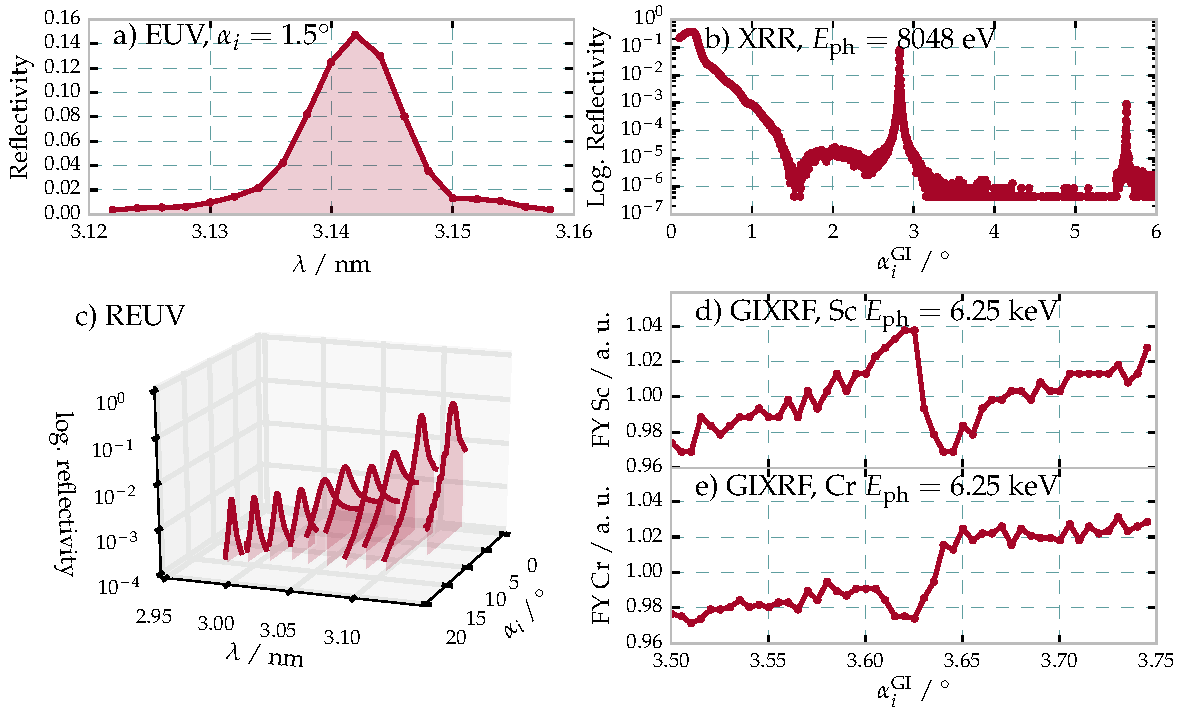
\includegraphics[width=\textwidth]{img/CrSc_all_data}
  \caption{Full data set used in the combined analysis. Due to redundancy, the \gls{xrf} data for the Sc at a photon energy of $E_\text{ph}=\ev{5500}$ was omitted.}
  \label{ch_spec:fig_CrSc_all_data}
\end{figure*}

As in the combined analysis conducted for the Mo/Si/C systems in Sec.~\ref{ch_spec:sec_MoSi_euv_xrr_combined}, we define the minimization functional for the combined analysis of all the datasets as
\begin{align}
\chi^2 = \tilde{\chi}^2_\text{EUV} +\tilde{\chi}^2_\text{XRR} 
+\tilde{\chi}^2_\text{REUV} + 
\tilde{\chi}^2_\text{GIXRF(Sc)}+\tilde{\chi}^2_\text{GIXRF(Cr)}\text{,} 
\label{ch_spec:eqn_CrSc_total_chi_2}
\end{align}
where each of the reduced functionals is defined as
\begin{align}
\tilde{\chi}^2 = \frac{1}{M - P} \bigg[\sum\limits_{m} \frac{(I_m^\text{model} 
- I_m^\text{meas})^2}{\tilde{\sigma}_m^2} \bigg] \text{,} 
\label{ch_spec:eqn_CrSc_reduced_chi_2}
\end{align}
with $M$ being the number of measurement points in each experiment and $P$ the 
number of parameters for the model. Statistical and systematic uncertainties 
for each data point are included in $\tilde{\sigma}_m$. The definition of 
Eq.~\eqref{ch_spec:eqn_CrSc_total_chi_2} ensures that all experiments are weighted equally 
considering their respective uncertainties. This functional corresponds to the combined $\chi^2$ functional defined in \eqref{ch_spec:eqn_Mo_Si_C_total_chi_2}, augmented by the additional measurements conducted here.

Firstly, similar as for the other two sample systems treated in this chapter, the parameters of the model, here the gradual interface model with the parameters and their limits listed in table~\ref{ch_spec:tbl_CrSc_gradual_parametrization}, were obtained using the \gls{pso} method to find a solution reproducing the experimental results. Secondly, following the maximum likelihood approach employing the \gls{mcmc} method as detailed in Sec.~\ref{ch_spec:sec_maximum_likelihood}, starting from this the uniqueness and confidence intervals for each parameter were obtained. The \gls{pso} result was further refined by taking the $50\%$ percentile of the resulting likelihood distribution for each parameter.

Through the minimization of the combined $\chi^2$ functional in Eq.~\eqref{ch_spec:eqn_CrSc_total_chi_2} via the \gls{pso} method, the best model parameters were obtained. It should be noted here, that in case of the \gls{xrr} curve, the analyzed data set was restricted to the two visible Bragg peaks which contain the information on the periodic part of the layer system. The data in between those does reflect the top surface layer thicknesses and was therefore analyzed separately to obtain the capping layer thicknesses after the optimization of the periodic part. The results for the capping layer thicknesses listed in table~\ref{ch_spec:tbl_CrSc_best_model_capping} was consequently used throughout the theoretical analysis for all experiments described here.
\begin{table}[htbp]
\centering
\caption{Optimized model parameters obtained by \gls{pso} analysis}
\label{ch_spec:tbl_CrSc_best_model_capping}
\begin{tabular}{@{}ll@{}}
\toprule
Parameter &  \gls{xrr} (areas in between the peaks)\\ \midrule
$d_\text{C (cap)}$ / nm  & $0.709$ \\ 
$d_\text{CrO (cap)}$ / nm  & $0.913$ \\ 
$d_\text{Cr (cap)}$ / nm  & $ 2.495$ \\ 
$\rho_\text{C (cap)}$ & $0.527$\\ 
$\rho_\text{CrO (cap)}$& $0.548$\\
$\rho_\text{Cr (cap)}$ & $0.791$\\
 \bottomrule
\end{tabular}
\end{table}

\subsubsection{Confidence Intervals and Evaluation of the Experimental Methods}
As discussed numerously throughout this chapter, the single optimization based on an \gls{pso} result ideally delivers a global minimum of the respective optimization functional. However, no information is obtained about the uniqueness and accuracy of the solution or correlation of parameters causing ambiguity of the results. Consequently, in addition to fitting the data with a particle swarm optimizer, each result was verified based on the \gls{mcmc} method described above to evaluate the confidence intervals for each parameter. To assess the performance of each of the experimental methods individually, the two step process, i.e.~the \gls{pso} fitting procedure followed by the \gls{mcmc} sampling, was conducted for each standalone experiment as well as for the combined optimization problem stated in Eq.~\eqref{ch_spec:eqn_CrSc_total_chi_2}.

The results are compiled in Table \ref{ch_spec:tbl_CrSc_MCMC_results}. The confidence intervals were calculated by evaluating the probability distribution as a result of the \gls{mcmc} procedure for each parameter around its \gls{pso} fit results. The confidence intervals given here represent percentiles of the number of samples found in the interval defined by the upper and lower bounds used for the \gls{pso} procedure for each parameter. In the case of 
a centered Gaussian distribution, percentiles of $2.3\%$ and $97.8\%$ of the integrated number of samples forming the distribution, mark the interval of four times the standard deviation, i.e.~$\pm 2\sigma$ in statistical terms. Due to potential asymmetries in the actual distributions found by the \gls{mcmc} method, explicit upper and lower bounds of the confidence intervals are given in table \ref{ch_spec:tbl_CrSc_MCMC_results} based on these percentiles. The best model value is based on the \gls{pso} fit result and is refined by the \gls{mcmc} sampling by calculating the mean value, i.e.~the 50\% percentile, of the distribution of samples following the \gls{mcmc} procedure.
\begin{table*}
\centering
\caption{Optimized model parameters with confidence intervals derived from MCMC 
validation for each individual experiment and the combined analysis}
\label{ch_spec:tbl_CrSc_MCMC_results}
\begin{tabular}{@{}llllll@{}}
\toprule
Parameter &  Combined & EUV  & XRR  & REUV  & GIXRF\\ \midrule
$D$ / nm& $1.5737_{-0.0010}^{+0.0008}$ & $1.5749_{-0.0022}^{+0.0014}$ & 
$1.5726_{-0.0042}^{+0.0035}$& $1.5728_{-0.0019}^{+0.0016}$& 
$1.5741_{-0.0024}^{+0.0021}$ \\ \addlinespace
$\Gamma_{Sc}$ & $0.48_{-0.04}^{+0.04}$ & $0.35_{-0.11}^{+0.14}$ & 
$0.42_{-0.26}^{+0.35}$& $0.52_{-0.07}^{+0.09}$& $0.49_{-0.10}^{+0.09}$ \\ 
\addlinespace
$s_d$ / nm& $1.34_{-0.26}^{+0.18}$ & $0.72_{-0.66}^{+0.67}$ & 
$0.60_{-0.57}^{+0.78}$& $0.89_{-0.83}^{+0.59}$& $1.27_{-0.38}^{+0.24}$ \\ 
\addlinespace
$\Gamma_\sigma$ & $0.16_{-0.16}^{+0.51}$ & $0.29_{-0.28}^{+0.64}$ & 
$0.40_{-0.39}^{+0.57}$& $0.33_{-0.32}^{+0.61}$& $0.39_{-0.37}^{+0.57}$ \\ 
\addlinespace
$\eta$ & $0.56_{-0.16}^{+0.06}$ & $0.44_{-0.30}^{+0.16}$ & 
$0.38_{-0.36}^{+0.33}$& $0.52_{-0.37}^{+0.14}$& $0.37_{-0.34}^{+0.25}$ \\ 
\addlinespace
$\sigma_r$ / nm& $0.11_{-0.10}^{+0.11}$ & $0.17_{-0.15}^{+0.12}$ & 
$0.13_{-0.12}^{+0.14}$& $0.17_{-0.16}^{+0.16}$& $0.27_{-0.25}^{+0.20}$ \\ 
\addlinespace
$\rho_{Sc}$ & $0.94_{-0.12}^{+0.05}$ & $0.84_{-0.32}^{+0.15}$ & 
$0.78_{-0.27}^{+0.21}$& $0.94_{-0.14}^{+0.06}$& $0.83_{-0.30}^{+0.17}$ \\ 
\addlinespace
$\rho_{Cr}$ & $0.98_{-0.08}^{+0.02}$ & $0.96_{-0.13}^{+0.04}$ & 
$0.83_{-0.27}^{+0.16}$& $0.90_{-0.21}^{+0.09}$& $0.86_{-0.28}^{+0.14}$ \\ 
\addlinespace
 \bottomrule
\end{tabular}
\end{table*}

\begin{figure*}[htbp]
  \centering
  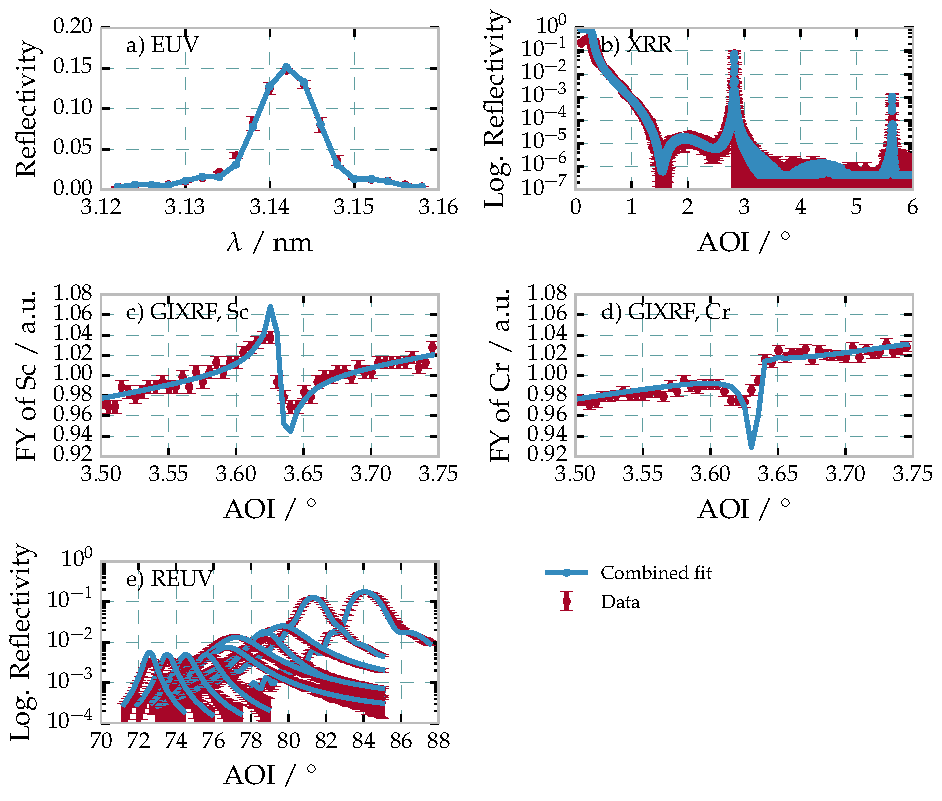
\includegraphics[width=\textwidth]{img/CrSc_combined_fit_result}
  \caption{Measured reflectance and fluorescence yield curves in direct comparison with the calculated reflectance and intensity curves for the 
optimized parameters obtained through the combined analysis of all experiments as listed in 
table~\ref{ch_spec:tbl_CrSc_MCMC_results}.}
  \label{ch_spec:fig_combined_fit_result}
\end{figure*}
Before discussing the achieved reconstruction and the corresponding confidence intervals of each of the methods in detail, we shall view the theoretical curves calculated from the best model of the combined analysis. The curves are shown in direct comparison with the data from Fig.~\ref{ch_spec:fig_CrSc_all_data} including the respective experimental uncertainties in Fig.~\ref{ch_spec:fig_combined_fit_result}. Clearly, the data and the solution found in the optimization procedure show excellent agreement indicating that the gradual interface model indeed provides a very good representation of physical reality with respect to the experiments conducted here. Nevertheless, differences can be observed. The reason lies 
in the fact that the model is potentially still too ideal. Small variations 
during the deposition process, for example, could lead to imperfections, which 
are not described in a strictly periodic model. However, including these by 
explicitly breaking the periodicity would again lead to an ill-defined model 
with a vastly increased number of parameters and is thus not practical. Another 
reason is the deviation in the homogeneity of the sample, e.g.~a varying period 
across the sample, which cause mismatches if the measurement position varies 
slightly between the different experimental setups. The latter effects were 
considered in the uncertainties of the individual measurements by measuring the 
EUV reflectivity at positions $\pm 2$ mm from the center position and fitting 
the model. The result was a $\Delta D = 2$ pm shift in the period over $4$ mm 
across the sample.


\paragraph{Parameter correlations in the combined analysis}
With the optimized model parameters listed in table~\ref{ch_spec:tbl_CrSc_MCMC_results} and shown in Fig.~\ref{ch_spec:fig_combined_fit_result} for the combined analysis, a model reconstruction could be obtained explaining the data for each of the experiments. The \gls{mcmc} sampling of the likelihood functional based on the $\chi^2$ definition in Eq.~\eqref{ch_spec:eqn_CrSc_total_chi_2} yields the corresponding confidence intervals for all parameters and experiments given through the upper and lower bound as described above. Here, we shall illustrate and discuss in detail the resulting likelihood distributions obtained from the combined analysis, as they show that correlations of the parameters could be resolved and only persist for a single important case. For that, Fig.~\ref{ch_spec:fig_CrSc_cornerplot_combined} shows the full matrix of two- and one-dimensional likelihood distribution projections marginalizing over all other parameters. The details of how this figure is to be interpreted are described in detail above in Sec.~\ref{ch_spec:sec_maximum_likelihood} for the example of Mo and Si layer thicknesses obtained through fitting \gls{euv} reflectivity data.
\begin{figure*}[htbp]
  \centering
  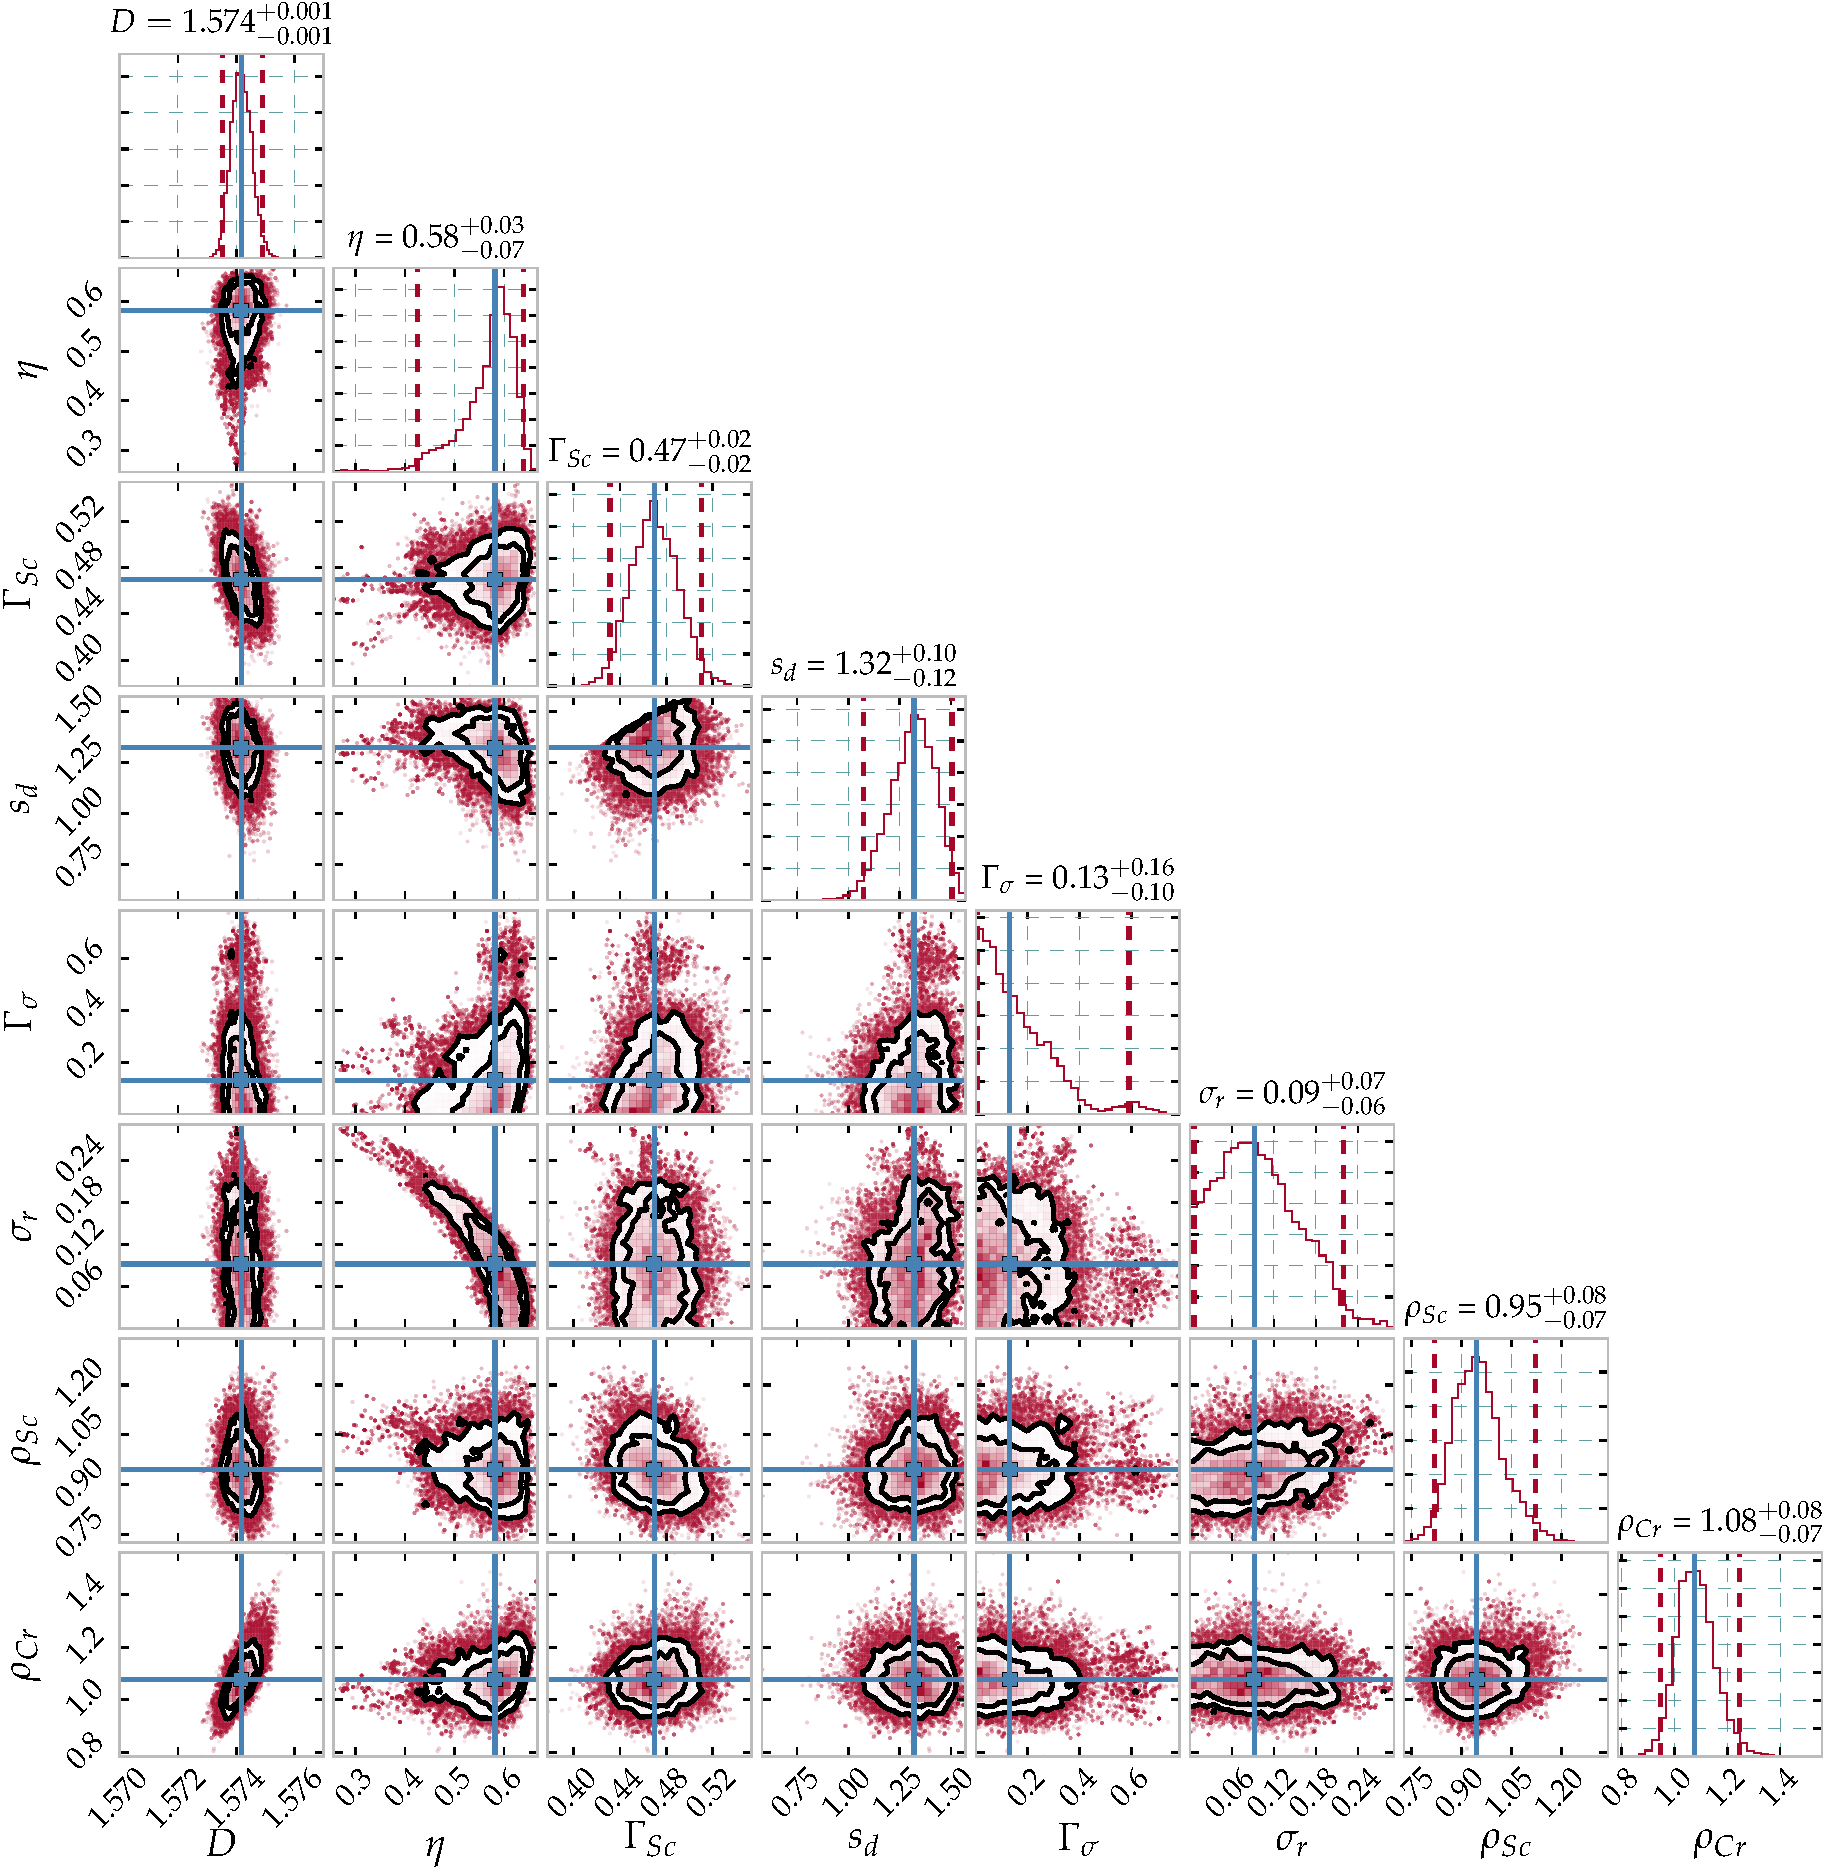
\includegraphics[width=\textwidth]{img/CrSc_cornerplot_combined}
  \caption{Matrix representation of the result of the maximum likelihood analysis based on the \gls{mcmc} method for all parameter combinations. At the top of each column, the one-dimensional projection of the likelihood distribution for the respective parameter is shown in analogy to the figures \ref{ch_spec:fig_Mo_Si_C_d_Mo_vs_d_Si} or \ref{ch_spec:fig_ptb17_MCMC_other_params}. The dotted red lines indicate the $\pm 2 \sigma$ interval, i.e.~two standard deviations from the center value ($\SI{50}{\percent}$ percentile). The latter is indicated through the solid blue lines. In the two dimensional projections, the solid black contours mark the areas for one and two standard deviations, respectively. For a discussion of the observed features see main text}
  \label{ch_spec:fig_CrSc_cornerplot_combined}
\end{figure*}
Here, all possible gradual interface model parameter combinations are shown as two dimensional histograms together with the one-dimensional projection at the diagonal of the plot matrix. The solid blue line represents the values of the optimized model after both, the \gls{pso} and refining through the \gls{mcmc} method. They correspond to the values listed in table~\ref{ch_spec:tbl_CrSc_MCMC_results} for the combined analysis column.

Generally, most of the parameter combinations do not show distinct correlations but approach the shape of a two-dimensional Gaussian distribution, which would be expected for a unique solution with corresponding uncertainty. It should be noted that in some cases, the distribution is truncated by parameter limits, which follow from physical or mathematical restrictions on the parameters as discussed in Sec.~\ref{ch_spec:sec_CrSc_gradual_model}, such as for the densities $\rho_\text{Sc}$ and $\rho_\text{Cr}$ as well as for the interface region ratio $\Gamma_\sigma$. In addition, the latter parameter shows a bimodal distribution for all two-dimensional histograms with clear emphasis on the lower value. That is a particularly interesting result of the combined analysis as it clearly demonstrates that only strongly asymmetric interface regions are minimizing the $\chi^2$ functional and it may thus be concluded that this corresponds to the physical reality in the sample.

Finally, the parameter set of the \gls{rms} roughness $\sigma_r$ and the interdiffusion parameter $\eta$ show a ``banana shaped'' correlation significantly broadening the confidence intervals for both parameters. Fig.~\ref{ch_spec:fig_CrSc_eta_rho_correlation} shows a magnification of that particular histogram to better illustrate this property.
\begin{figure}[htbp]
  \centering
  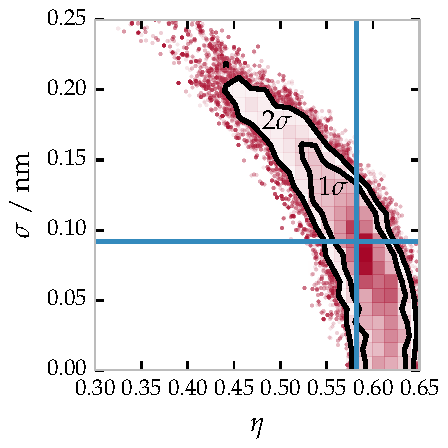
\includegraphics{img/CrSc_eta_rho_correlation}
  \caption{Magnified two dimensional projection histogram for the correlation of the interdiffusion parameter $\eta$ and the \gls{rms} roughness parameter $\sigma_r$ from Fig.~\ref{ch_spec:fig_CrSc_cornerplot_combined}. Again, the areas of one and two standard deviations are indicated together with the $\SI{50}{\percent}$ percentile as solid blue lines.}
  \label{ch_spec:fig_CrSc_eta_rho_correlation}
\end{figure}
The broad spectrum of values covered by the distribution in both parameters hints at a indistinguishability of those two model parameters, and consequently physical properties of the sample, based on the analyzed data. In fact, this conclusion can easily be understood as none of the applied experimental methods can separate the effect of roughness and interdiffusion. For better understanding this, we shall consider the relatively large beam footprint, with the smallest one of all experiments covering and area of approximately \mm{1} by \mm{1}, in comparison to the roughness dimensions and frequencies expected in the order of nanometers. Thereby, any reflected radiation or fluorescence radiation excited within the multilayer always represents an average of the rough interface morphology. That, however, can not be distinguished from a homogeneous layer with gradual interdiffusion along the surface normal of the sample. The solution to this problem of distinction is the analysis of diffuse scattering from the sample in addition to the combined analysis, which is the topic of the Ch.~\ref{ch_diff} of this thesis.

\paragraph{Confidence intervals depending on the employed method}
The confidence intervals of each experimental method differ significantly as table~\ref{ch_spec:tbl_CrSc_MCMC_results} shows. The reason behind this is the different sensitivity of the methods to the specific physical properties described by the respective model parameter. To better illustrate the information compiled in the table above, for each method and each parameter the total confidence interval is shown in Fig.~\ref{fig:confidence_intervals} in a radial plot. The total confidence interval is defined as the difference of the upper and lower values as listed in table~\ref{ch_spec:tbl_CrSc_MCMC_results} for each experiment and parameter.
\begin{figure}[htbp]
  \centering
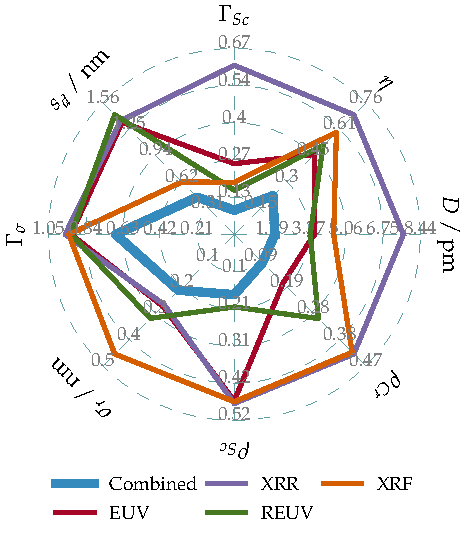
\includegraphics{img/CrSc_confidence_intervals_radar}
  \caption{Visual representation of the total confidence intervals for each of 
the parameters with respect to each of the individual experiments as well as 
the combined analysis.}
  \label{fig:confidence_intervals}
\end{figure}
The plot shows the four relevant experiments and the combined analysis results. Any value closer to the origin of the radial plot indicates a smaller confidence interval and thus a better accuracy of the solution found for the respective parameter.

It is worth noting that the confidence interval for the combined analysis is 
significantly smaller compared to the individual experiments for all parameters and therefore yields the best result. This is especially true for the parameter $\Gamma_\sigma$ describing the asymmetry of the interdiffusion layers. Within each of the individual experiments this parameter has a large uncertainty and can not be determined, whereas the combined analysis delivers a significant result of a clearly asymmetric interdiffusion layer thickness. In combination with the observations made above for the respective histograms in Fig.~\ref{ch_spec:fig_CrSc_cornerplot_combined}, we can conclude that this asymmetry is indeed a significant result and that the remaining fairly large confidence interval mainly results from the fact of having a bimodal distribution as the dotted lines in the respective histogram Fig.~\ref{ch_spec:fig_CrSc_cornerplot_combined} prove. A possible explanation for this asymmetry is the deposition process through magnetron sputtering. The elements Cr and Sc have different mass and thus different momentum when deposited onto each other. A similar effect is known from the deposition of Mo/Si multilayer systems, where the heavier Mo shows higher penetration into the Si layer than vice versa \cite{petford-long_highresolution_1987}. In the case of Cr/Sc multilayers, the Cr is heavier and thus has higher momentum leading to a broader interdiffusion layer, which is indeed also the interface region found to be the broadest by the analysis conducted here.

The final result of this analysis of Cr/Sc multilayer systems with sub-nanometer layer thicknesses is shown in Fig.~\ref{ch_spec:fig_CrSc_electron_density_profile} by the depth dependence of the index of refraction in direct comparison with the initial binary model.
\begin{figure}[htbp]
  \centering
  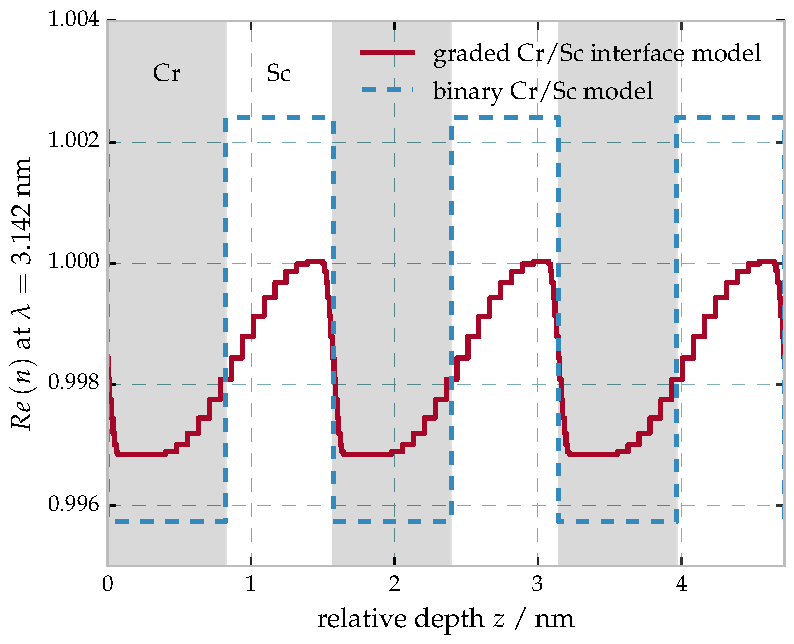
\includegraphics[width=0.7\textwidth]{img/CrSc_binary_vs_fitted_gradual_model}
  \caption{Real part of the index of refraction $n$  based on the results of 
the optimized parameters listed in Table~\ref{tbl:results} for the combined 
analysis for a selected wavelength. The gradual interface model is shown in 
direct comparison to the binary model optimized for the EUV reflectance curve 
over three full periods. The resulting strong asymmetry in the width of the 
interface regions is clearly visible (see text). The gray and white shaded 
areas indicate the Cr and Sc layers, respectively, for the binary model.}
  \label{ch_spec:fig_CrSc_electron_density_profile}
\end{figure}
As mentioned before, the most remarkable result of the combined analysis is the strong asymmetry of the interdiffusion layers. This can only be shown by the combination of all 
analytical experiments conducted here. In addition, the comparison shows that at no point within the periodic multilayer stack pure Sc or pure Cr layers are observed, but always a mixture of both. In the context of answering the question of poor reflectivity with respect to the theoretical possible maximum, this shows that interdiffusion may be the main reason. The loss of contrast with respect to the binary model indicated, causes the diminished reflectivity. We should note, however, that due to the correlation between roughness and interdiffusion this result is still to be verified by the aforementioned analysis of diffuse scattering. This is the topic of chapter~\ref{ch_diff}.

The experiments, methods and findings of this section are part of the publication \fullcite{haase_multiparameter_2016}


